%%=============================================================================
%% LaTeX sjabloon voor bachelorproef, HoGent Bedrijf en Organisatie
%% Opleiding Toegepaste Informatica
%%=============================================================================

\documentclass[fleqn,a4paper,12pt]{book}

%%=============================================================================
%% LaTeX sjabloon voor de bachelorproef, HoGent Bedrijf en Organisatie
%% Opleiding toegepaste informatica
%%
%% Structuur en algemene vormgeving. Meestal hoef je hier niets te wijzigen.
%%
%% Vormgeving gebaseerd op "The Legrand Orange Book", version 2.0 (9/2/15)
%% door Mathias Legrand (legrand.mathias@gmail.com) met aanpassingen door
%% Vel (vel@latextemplates.com). Het oorspronkelijke template is te vinden op
%% http://www.LaTeXTemplates.com
%%
%% Aanpassingen voor HoGent toegepaste informatica: 
%%   Bert Van Vreckem <bert.vanvreckem@hogent.be>
%% Licentie: 
%%   CC BY-NC-SA 3.0 (http://creativecommons.org/licenses/by-nc-sa/3.0/)
%%=============================================================================

%%-----------------------------------------------------------------------------
%% Packages
%%-----------------------------------------------------------------------------

\usepackage[top=3cm,bottom=3cm,left=3cm,right=3cm,headsep=10pt,a4paper]{geometry} % Page margins
\usepackage[utf8]{inputenc}  % Accenten gebruiken in tekst (vb. é ipv \'e)
\usepackage{amsfonts}        % AMS math packages: extra wiskundige
\usepackage{amsmath}         %   symbolen (o.a. getallen-
\usepackage{amssymb}         %   verzamelingen N, R, Z, Q, etc.)
\usepackage[english,dutch]{babel}    % Taalinstellingen: woordsplitsingen,
                             %  commando's voor speciale karakters
                             %  ("dutch" voor NL)
\usepackage{iflang}
\usepackage{eurosym}         % Euro-symbool €
\usepackage{geometry}
\usepackage{graphicx}        % Invoegen van tekeningen
\graphicspath{{img/}}       % Specifies the directory where pictures are stored
\usepackage{tikz}            % Required for drawing custom shapes
\usepackage[pdftex,bookmarks=true]{hyperref}
                             % PDF krijgt klikbare links & verwijzingen,
                             %  inhoudstafel
\usepackage{enumitem}        % Customize lists
\setlist{nolistsep}         % Reduce spacing between list items
\usepackage{listings}        % Broncode mooi opmaken
\usepackage{multirow}        % Tekst over verschillende cellen in tabellen
\usepackage{rotating}        % Tabellen en figuren roteren

\usepackage{booktabs}        % Required for nicer horizontal rules in tables

\usepackage{xcolor}          % Required for specifying colors by name
\definecolor{maincolor}{RGB}{0,147,208} % Define the main color used for 
                             % highlighting throughout the book
                             % 0, 147, 208 = officiële kleur HoGent FBO

% Paragraph style: no indent, add space between paragraphs
\setlength{\parindent}{0em}
\setlength{\parskip}{1em}

\usepackage{etoolbox}
\usepackage{titling} % Macros for title, author, etc
\usepackage{lipsum}          % Voor vultekst (lorem ipsum)


\usepackage{subcaption}


%----------------------------------------------------------------------------------------
%	FONTS
%----------------------------------------------------------------------------------------

\usepackage{avant} % Use the Avantgarde font for headings
%\usepackage{times} % Use the Times font for headings
\usepackage{mathptmx} % Use the Adobe Times Roman as the default text font together with math symbols from the Sym­bol, Chancery and Com­puter Modern fonts

\usepackage{microtype} % Slightly tweak font spacing for aesthetics
\usepackage[utf8]{inputenc} % Required for including letters with accents
\usepackage[T1]{fontenc} % Use 8-bit encoding that has 256 glyphs

%------------------------------------------------------------------------------
%	TITLE PAGE
%------------------------------------------------------------------------------

\newcommand{\inserttitlepage}{%
\begin{titlepage}
  \newgeometry{top=2cm,bottom=1.5cm,left=1.5cm,right=1.5cm}
  \begin{center}

    \begingroup
    \rmfamily
    
\includegraphics[width=2.5cm]{img/HG-beeldmerk-woordmerk}\\[.5cm]
    Faculteit Bedrijf en Organisatie\\[3cm]
    \titel
    \vfill
    \student\\[3.5cm]
    Scriptie voorgedragen tot het bekomen van de graad van\\professionele bachelor in de toegepaste informatica\\[2cm]
    Promotor:\\
    \promotor\\
    \ifdefempty{\copromotor}{\vspace{2.5cm}}{Co-promotor:\\\copromotor\\[2.5cm]}
    Instelling: \instelling\\[.5cm]
    Academiejaar: \academiejaar\\[.5cm]
    \ifcase \examenperiode \or Eerste \or Tweede \else Derde \fi examenperiode
    \endgroup

  \end{center}
  \restoregeometry
\end{titlepage}
  \emptypage
\begin{titlepage}
  \newgeometry{top=5.35cm,bottom=1.5cm,left=1.5cm,right=1.5cm}
  \begin{center}

    \begingroup
    \rmfamily
    \IfLanguageName{dutch}{Faculteit Bedrijf en Organisatie}{Faculty of Business and Information Management}\\[3cm]
    \titel
    \vfill
    \student\\[3.5cm]
    \IfLanguageName{dutch}{Scriptie voorgedragen tot het bekomen van de graad van\\professionele bachelor in de toegepaste informatica}{Thesis submitted in partial fulfilment of the requirements for the degree of\\professional bachelor of applied computer science}\\[2cm]
    Promotor:\\
    \promotor\\
    \ifdefempty{\copromotor}{\vspace{2.5cm}}{Co-promotor:\\\copromotor\\[2.5cm]}
    \IfLanguageName{dutch}{Instelling}{Institution}: \instelling\\[.5cm]
    \IfLanguageName{dutch}{Academiejaar}{Academic year}: \academiejaar\\[.5cm]
    \IfLanguageName{dutch}{%
    \ifcase \examenperiode \or Eerste \or Tweede \else Derde \fi examenperiode}{%
    \ifcase \examenperiode \or First \or Second \else Third \fi examination period}
    \endgroup

  \end{center}
  \restoregeometry
\end{titlepage}
}

%----------------------------------------------------------------------------------------
%	BIBLIOGRAPHY AND INDEX
%----------------------------------------------------------------------------------------

\usepackage[style=apa,backend=biber]{biblatex}
\usepackage{csquotes}
\DeclareLanguageMapping{dutch}{dutch-apa}
\addbibresource{bachproef-tin.bib} % BibTeX bibliography file
\addbibresource{../voorstel/voorstel.bib}
\defbibheading{bibempty}{}

\usepackage{calc} % For simpler calculation - used for spacing the index letter headings correctly
\usepackage{makeidx} % Required to make an index
\makeindex % Tells LaTeX to create the files required for indexing

%----------------------------------------------------------------------------------------
%	MAIN TABLE OF CONTENTS
%----------------------------------------------------------------------------------------

\usepackage{titletoc} % Required for manipulating the table of contents

\contentsmargin{0cm} % Removes the default margin

% Part text styling
\titlecontents{part}[0cm]
{\addvspace{20pt}\centering\large\bfseries}
{}
{}
{}

% Chapter text styling
\titlecontents{chapter}[1.25cm] % Indentation
{\addvspace{12pt}\large\sffamily\bfseries} % Spacing and font options for chapters
{\color{maincolor!60}\contentslabel[\Large\thecontentslabel]{1.25cm}\color{maincolor}} % Chapter number
{\color{maincolor}}
{\color{maincolor!60}\normalsize\;\titlerule*[.5pc]{.}\;\thecontentspage} % Page number

% Section text styling
\titlecontents{section}[1.25cm] % Indentation
{\addvspace{3pt}\sffamily\bfseries} % Spacing and font options for sections
{\contentslabel[\thecontentslabel]{1.25cm}} % Section number
{}
{\hfill\color{black}\thecontentspage} % Page number
[]

% Subsection text styling
\titlecontents{subsection}[1.25cm] % Indentation
{\addvspace{1pt}\sffamily\small} % Spacing and font options for subsections
{\contentslabel[\thecontentslabel]{1.25cm}} % Subsection number
{}
{\ \titlerule*[.5pc]{.}\;\thecontentspage} % Page number
[]

% List of figures
\titlecontents{figure}[0em]
{\addvspace{-5pt}\sffamily}
{\thecontentslabel\hspace*{1em}}
{}
{\ \titlerule*[.5pc]{.}\;\thecontentspage}
[]

% List of tables
\titlecontents{table}[0em]
{\addvspace{-5pt}\sffamily}
{\thecontentslabel\hspace*{1em}}
{}
{\ \titlerule*[.5pc]{.}\;\thecontentspage}
[]

%----------------------------------------------------------------------------------------
%	MINI TABLE OF CONTENTS IN PART HEADS
%----------------------------------------------------------------------------------------

% Chapter text styling
\titlecontents{lchapter}[0em] % Indenting
{\addvspace{15pt}\large\sffamily\bfseries} % Spacing and font options for chapters
{\color{maincolor}\contentslabel[\Large\thecontentslabel]{1.25cm}\color{maincolor}} % Chapter number
{}
{\color{maincolor}\normalsize\sffamily\bfseries\;\titlerule*[.5pc]{.}\;\thecontentspage} % Page number

% Section text styling
\titlecontents{lsection}[0em] % Indenting
{\sffamily\small} % Spacing and font options for sections
{\contentslabel[\thecontentslabel]{1.25cm}} % Section number
{}
{}

% Subsection text styling
\titlecontents{lsubsection}[.5em] % Indentation
{\normalfont\footnotesize\sffamily} % Font settings
{}
{}
{}

%----------------------------------------------------------------------------------------
%	PAGE HEADERS
%----------------------------------------------------------------------------------------

\usepackage{fancyhdr} % Required for header and footer configuration

\pagestyle{fancy}
\renewcommand{\chaptermark}[1]{\markboth{\sffamily\normalsize\bfseries\chaptername\ \thechapter.\ #1}{}} % Chapter text font settings
\renewcommand{\sectionmark}[1]{\markright{\sffamily\normalsize\thesection\hspace{5pt}#1}{}} % Section text font settings
\fancyhf{} \fancyhead[LE,RO]{\sffamily\normalsize\thepage} % Font setting for the page number in the header
\fancyhead[LO]{\rightmark} % Print the nearest section name on the left side of odd pages
\fancyhead[RE]{\leftmark} % Print the current chapter name on the right side of even pages
\renewcommand{\headrulewidth}{0.5pt} % Width of the rule under the header
\addtolength{\headheight}{2.5pt} % Increase the spacing around the header slightly
\renewcommand{\footrulewidth}{0pt} % Removes the rule in the footer
\fancypagestyle{plain}{\fancyhead{}\renewcommand{\headrulewidth}{0pt}} % Style for when a plain pagestyle is specified

% Removes the header from odd empty pages at the end of chapters
\makeatletter
\renewcommand{\cleardoublepage}{
\clearpage\ifodd\c@page\else
\hbox{}
\vspace*{\fill}
\thispagestyle{empty}
\newpage
\fi}

%----------------------------------------------------------------------------------------
%	THEOREM STYLES
%----------------------------------------------------------------------------------------

\usepackage{amsmath,amsfonts,amssymb,amsthm} % For math equations, theorems, symbols, etc

\newcommand{\intoo}[2]{\mathopen{]}#1\,;#2\mathclose{[}}
\newcommand{\ud}{\mathop{\mathrm{{}d}}\mathopen{}}
\newcommand{\intff}[2]{\mathopen{[}#1\,;#2\mathclose{]}}
\newtheorem{notation}{Notation}[chapter]

% Boxed/framed environments
\newtheoremstyle{maincolornumbox}% % Theorem style name
{0pt}% Space above
{0pt}% Space below
{\normalfont}% % Body font
{}% Indent amount
{\small\bf\sffamily\color{maincolor}}% % Theorem head font
{\;}% Punctuation after theorem head
{0.25em}% Space after theorem head
{\small\sffamily\color{maincolor}\thmname{#1}\nobreakspace\thmnumber{\@ifnotempty{#1}{}\@upn{#2}}% Theorem text (e.g. Theorem 2.1)
\thmnote{\nobreakspace\the\thm@notefont\sffamily\bfseries\color{black}---\nobreakspace#3.}} % Optional theorem note
\renewcommand{\qedsymbol}{$\blacksquare$}% Optional qed square

\newtheoremstyle{blacknumex}% Theorem style name
{5pt}% Space above
{5pt}% Space below
{\normalfont}% Body font
{} % Indent amount
{\small\bf\sffamily}% Theorem head font
{\;}% Punctuation after theorem head
{0.25em}% Space after theorem head
{\small\sffamily{\tiny\ensuremath{\blacksquare}}\nobreakspace\thmname{#1}\nobreakspace\thmnumber{\@ifnotempty{#1}{}\@upn{#2}}% Theorem text (e.g. Theorem 2.1)
\thmnote{\nobreakspace\the\thm@notefont\sffamily\bfseries---\nobreakspace#3.}}% Optional theorem note

\newtheoremstyle{blacknumbox} % Theorem style name
{0pt}% Space above
{0pt}% Space below
{\normalfont}% Body font
{}% Indent amount
{\small\bf\sffamily}% Theorem head font
{\;}% Punctuation after theorem head
{0.25em}% Space after theorem head
{\small\sffamily\thmname{#1}\nobreakspace\thmnumber{\@ifnotempty{#1}{}\@upn{#2}}% Theorem text (e.g. Theorem 2.1)
\thmnote{\nobreakspace\the\thm@notefont\sffamily\bfseries---\nobreakspace#3.}}% Optional theorem note

% Non-boxed/non-framed environments
\newtheoremstyle{maincolornum}% % Theorem style name
{5pt}% Space above
{5pt}% Space below
{\normalfont}% % Body font
{}% Indent amount
{\small\bf\sffamily\color{maincolor}}% % Theorem head font
{\;}% Punctuation after theorem head
{0.25em}% Space after theorem head
{\small\sffamily\color{maincolor}\thmname{#1}\nobreakspace\thmnumber{\@ifnotempty{#1}{}\@upn{#2}}% Theorem text (e.g. Theorem 2.1)
\thmnote{\nobreakspace\the\thm@notefont\sffamily\bfseries\color{black}---\nobreakspace#3.}} % Optional theorem note
\renewcommand{\qedsymbol}{$\blacksquare$}% Optional qed square
\makeatother

% Defines the theorem text style for each type of theorem to one of the three styles above
\newcounter{dummy}
\numberwithin{dummy}{section}
\theoremstyle{maincolornumbox}
\newtheorem{theoremeT}[dummy]{Theorem}
\newtheorem{problem}{Problem}[chapter]
\newtheorem{exerciseT}{Exercise}[chapter]
\theoremstyle{blacknumex}
\newtheorem{exampleT}{Example}[chapter]
\theoremstyle{blacknumbox}
\newtheorem{vocabulary}{Vocabulary}[chapter]
\newtheorem{definitionT}{Definition}[section]
\newtheorem{corollaryT}[dummy]{Corollary}
\theoremstyle{maincolornum}
\newtheorem{proposition}[dummy]{Proposition}

%----------------------------------------------------------------------------------------
%	DEFINITION OF COLORED BOXES
%----------------------------------------------------------------------------------------

\RequirePackage[framemethod=default]{mdframed} % Required for creating the theorem, definition, exercise and corollary boxes

% Theorem box
\newmdenv[skipabove=7pt,
skipbelow=7pt,
backgroundcolor=black!5,
linecolor=maincolor,
innerleftmargin=5pt,
innerrightmargin=5pt,
innertopmargin=5pt,
leftmargin=0cm,
rightmargin=0cm,
innerbottommargin=5pt]{tBox}

% Exercise box
\newmdenv[skipabove=7pt,
skipbelow=7pt,
rightline=false,
leftline=true,
topline=false,
bottomline=false,
backgroundcolor=maincolor!10,
linecolor=maincolor,
innerleftmargin=5pt,
innerrightmargin=5pt,
innertopmargin=5pt,
innerbottommargin=5pt,
leftmargin=0cm,
rightmargin=0cm,
linewidth=4pt]{eBox}

% Definition box
\newmdenv[skipabove=7pt,
skipbelow=7pt,
rightline=false,
leftline=true,
topline=false,
bottomline=false,
linecolor=maincolor,
innerleftmargin=5pt,
innerrightmargin=5pt,
innertopmargin=0pt,
leftmargin=0cm,
rightmargin=0cm,
linewidth=4pt,
innerbottommargin=0pt]{dBox}

% Corollary box
\newmdenv[skipabove=7pt,
skipbelow=7pt,
rightline=false,
leftline=true,
topline=false,
bottomline=false,
linecolor=gray,
backgroundcolor=black!5,
innerleftmargin=5pt,
innerrightmargin=5pt,
innertopmargin=5pt,
leftmargin=0cm,
rightmargin=0cm,
linewidth=4pt,
innerbottommargin=5pt]{cBox}

% Creates an environment for each type of theorem and assigns it a theorem text style from the "Theorem Styles" section above and a colored box from above
\newenvironment{theorem}{\begin{tBox}\begin{theoremeT}}{\end{theoremeT}\end{tBox}}
\newenvironment{exercise}{\begin{eBox}\begin{exerciseT}}{\hfill{\color{maincolor}\tiny\ensuremath{\blacksquare}}\end{exerciseT}\end{eBox}}
\newenvironment{definition}{\begin{dBox}\begin{definitionT}}{\end{definitionT}\end{dBox}}
\newenvironment{example}{\begin{exampleT}}{\hfill{\tiny\ensuremath{\blacksquare}}\end{exampleT}}
\newenvironment{corollary}{\begin{cBox}\begin{corollaryT}}{\end{corollaryT}\end{cBox}}

%----------------------------------------------------------------------------------------
%	REMARK ENVIRONMENT
%----------------------------------------------------------------------------------------

\newenvironment{remark}{\par\vspace{10pt}\small % Vertical white space above the remark and smaller font size
\begin{list}{}{
\leftmargin=35pt % Indentation on the left
\rightmargin=25pt}\item\ignorespaces % Indentation on the right
\makebox[-2.5pt]{\begin{tikzpicture}[overlay]
\node[draw=maincolor!60,line width=1pt,circle,fill=maincolor!25,font=\sffamily\bfseries,inner sep=2pt,outer sep=0pt] at (-15pt,0pt){\textcolor{maincolor}{R}};\end{tikzpicture}} % Orange R in a circle
\advance\baselineskip -1pt}{\end{list}\vskip5pt} % Tighter line spacing and white space after remark

%----------------------------------------------------------------------------------------
%	SECTION NUMBERING IN THE MARGIN
%----------------------------------------------------------------------------------------

\makeatletter
\renewcommand{\@seccntformat}[1]{\llap{\textcolor{maincolor}{\csname the#1\endcsname}\hspace{1em}}}
\renewcommand{\section}{\@startsection{section}{1}{\z@}
{-4ex \@plus -1ex \@minus -.4ex}
{1ex \@plus.2ex }
{\normalfont\large\sffamily\bfseries}}
\renewcommand{\subsection}{\@startsection {subsection}{2}{\z@}
{-3ex \@plus -0.1ex \@minus -.4ex}
{0.5ex \@plus.2ex }
{\normalfont\sffamily\bfseries}}
\renewcommand{\subsubsection}{\@startsection {subsubsection}{3}{\z@}
{-2ex \@plus -0.1ex \@minus -.2ex}
{.2ex \@plus.2ex }
{\normalfont\small\sffamily\bfseries}}
\renewcommand\paragraph{\@startsection{paragraph}{4}{\z@}
{-2ex \@plus-.2ex \@minus .2ex}
{.1ex}
{\normalfont\small\sffamily\bfseries}}

%----------------------------------------------------------------------------------------
%	PART HEADINGS
%----------------------------------------------------------------------------------------

% numbered part in the table of contents
\newcommand{\@mypartnumtocformat}[2]{%
\setlength\fboxsep{0pt}%
\noindent\colorbox{maincolor!20}{\strut\parbox[c][.7cm]{\ecart}{\color{maincolor!70}\Large\sffamily\bfseries\centering#1}}\hskip\esp\colorbox{maincolor!40}{\strut\parbox[c][.7cm]{\linewidth-\ecart-\esp}{\Large\sffamily\centering#2}}}%
%%%%%%%%%%%%%%%%%%%%%%%%%%%%%%%%%%
% unnumbered part in the table of contents
\newcommand{\@myparttocformat}[1]{%
\setlength\fboxsep{0pt}%
\noindent\colorbox{maincolor!40}{\strut\parbox[c][.7cm]{\linewidth}{\Large\sffamily\centering#1}}}%
%%%%%%%%%%%%%%%%%%%%%%%%%%%%%%%%%%
\newlength\esp
\setlength\esp{4pt}
\newlength\ecart
\setlength\ecart{1.2cm-\esp}
\newcommand{\thepartimage}{}%
\newcommand{\partimage}[1]{\renewcommand{\thepartimage}{#1}}%
\def\@part[#1]#2{%
\ifnum \c@secnumdepth >-2\relax%
\refstepcounter{part}%
\addcontentsline{toc}{part}{\texorpdfstring{\protect\@mypartnumtocformat{\thepart}{#1}}{\partname~\thepart\ ---\ #1}}
\else%
\addcontentsline{toc}{part}{\texorpdfstring{\protect\@myparttocformat{#1}}{#1}}%
\fi%
\startcontents%
\markboth{}{}%
{\thispagestyle{empty}%
\begin{tikzpicture}[remember picture,overlay]%
\node at (current page.north west){\begin{tikzpicture}[remember picture,overlay]%
\fill[maincolor!20](0cm,0cm) rectangle (\paperwidth,-\paperheight);
\node[anchor=north] at (4cm,-3.25cm){\color{maincolor!40}\fontsize{220}{100}\sffamily\bfseries\@Roman\c@part};
\node[anchor=south east] at (\paperwidth-1cm,-\paperheight+1cm){\parbox[t][][t]{8.5cm}{
\printcontents{l}{0}{\setcounter{tocdepth}{1}}%
}};
\node[anchor=north east] at (\paperwidth-1.5cm,-3.25cm){\parbox[t][][t]{15cm}{\strut\raggedleft\color{white}\fontsize{30}{30}\sffamily\bfseries#2}};
\end{tikzpicture}};
\end{tikzpicture}}%
\@endpart}
\def\@spart#1{%
\startcontents%
\phantomsection
{\thispagestyle{empty}%
\begin{tikzpicture}[remember picture,overlay]%
\node at (current page.north west){\begin{tikzpicture}[remember picture,overlay]%
\fill[maincolor!20](0cm,0cm) rectangle (\paperwidth,-\paperheight);
\node[anchor=north east] at (\paperwidth-1.5cm,-3.25cm){\parbox[t][][t]{15cm}{\strut\raggedleft\color{white}\fontsize{30}{30}\sffamily\bfseries#1}};
\end{tikzpicture}};
\end{tikzpicture}}
\addcontentsline{toc}{part}{\texorpdfstring{%
\setlength\fboxsep{0pt}%
\noindent\protect\colorbox{maincolor!40}{\strut\protect\parbox[c][.7cm]{\linewidth}{\Large\sffamily\protect\centering #1\quad\mbox{}}}}{#1}}%
\@endpart}
\def\@endpart{\vfil\newpage
\if@twoside
\if@openright
\null
\thispagestyle{empty}%
\newpage
\fi
\fi
\if@tempswa
\twocolumn
\fi}

%----------------------------------------------------------------------------------------
%	CHAPTER HEADINGS
%----------------------------------------------------------------------------------------

% A switch to conditionally include a picture, implemented by  Christian Hupfer
\newif\ifusechapterimage
\usechapterimagetrue
\newcommand{\thechapterimage}{}%
\newcommand{\chapterimage}[1]{\ifusechapterimage\renewcommand{\thechapterimage}{#1}\fi}%
\def\@makechapterhead#1{%
{\parindent \z@ \raggedright \normalfont
\ifnum \c@secnumdepth >\m@ne
\if@mainmatter
\begin{tikzpicture}[remember picture,overlay]
\node at (current page.north west)
{\begin{tikzpicture}[remember picture,overlay]
\node[anchor=north west,inner sep=0pt] at (0,0) {\ifusechapterimage\includegraphics[width=\paperwidth]{\thechapterimage}\fi};
\draw[anchor=west] (\Gm@lmargin,-9cm) node [line width=2pt,rounded corners=15pt,draw=maincolor,fill=white,fill opacity=0.5,inner sep=15pt]{\strut\makebox[22cm]{}};
\draw[anchor=west] (\Gm@lmargin+.3cm,-9cm) node {\huge\sffamily\bfseries\color{black}\thechapter. #1\strut};
\end{tikzpicture}};
\end{tikzpicture}
\else
\begin{tikzpicture}[remember picture,overlay]
\node at (current page.north west)
{\begin{tikzpicture}[remember picture,overlay]
\node[anchor=north west,inner sep=0pt] at (0,0) {\ifusechapterimage\includegraphics[width=\paperwidth]{\thechapterimage}\fi};
\draw[anchor=west] (\Gm@lmargin,-9cm) node [line width=2pt,rounded corners=15pt,draw=maincolor,fill=white,fill opacity=0.5,inner sep=15pt]{\strut\makebox[22cm]{}};
\draw[anchor=west] (\Gm@lmargin+.3cm,-9cm) node {\huge\sffamily\bfseries\color{black}#1\strut};
\end{tikzpicture}};
\end{tikzpicture}
\fi\fi\par\vspace*{270\p@}}}

%-------------------------------------------

\def\@makeschapterhead#1{%
\begin{tikzpicture}[remember picture,overlay]
\node at (current page.north west)
{\begin{tikzpicture}[remember picture,overlay]
\node[anchor=north west,inner sep=0pt] at (0,0) {\ifusechapterimage\includegraphics[width=\paperwidth]{\thechapterimage}\fi};
\draw[anchor=west] (\Gm@lmargin,-9cm) node [line width=2pt,rounded corners=15pt,draw=maincolor,fill=white,fill opacity=0.5,inner sep=15pt]{\strut\makebox[22cm]{}};
\draw[anchor=west] (\Gm@lmargin+.3cm,-9cm) node {\huge\sffamily\bfseries\color{black}#1\strut};
\end{tikzpicture}};
\end{tikzpicture}
\par\vspace*{270\p@}}
\makeatother

%----------------------------------------------------------------------------------------
%	HYPERLINKS IN THE DOCUMENTS
%----------------------------------------------------------------------------------------

\usepackage{hyperref}
\hypersetup{hidelinks,backref=true,pagebackref=true,hyperindex=true,colorlinks=false,breaklinks=true,urlcolor= maincolor,bookmarks=true,bookmarksopen=false,pdftitle={Title},pdfauthor={Author}}
\usepackage{bookmark}
\bookmarksetup{
open,
numbered,
addtohook={%
\ifnum\bookmarkget{level}=0 % chapter
\bookmarksetup{bold}%
\fi
\ifnum\bookmarkget{level}=-1 % part
\bookmarksetup{color=maincolor,bold}%
\fi
}
}

%----------------------------------------------------------------------------------------
%	Java source code
%----------------------------------------------------------------------------------------

% Commando voor invoegen Java-broncodebestanden (dank aan Niels Corneille)
% Gebruik:
%   \codefragment{source/MijnKlasse.java}{Uitleg bij de code}
%
% Je kan dit aanpassen aan de taal die je zelf het meeste gebruikt in je
% bachelorproef.
\newcommand{\codefragment}[2]{ \lstset{%
  language=java,
  breaklines=true,
  float=th,
  caption={#2},
  basicstyle=\scriptsize,
  frame=single,
  extendedchars=\true
}
\lstinputlisting{#1}}

% Leeg blad
\newcommand{\emptypage}{%
\newpage
\thispagestyle{empty}
\mbox{}
\newpage
}


%%---------- Documenteigenschappen --------------------------------------------
%% TODO: Vul dit aan met je eigen info:

% Je eigen naam
\newcommand{\student}{Evert Vanderstadt}

% De naam van je promotor (lector van de opleiding)
\newcommand{\promotor}{Tom Antjon}

% De naam van je co-promotor. Als je promotor ook je opdrachtgever is en je
% dus ook inhoudelijk begeleidt (en enkel dan!), mag je dit leeg laten.
\newcommand{\copromotor}{Michiel Van Meervenne}

% Indien je bachelorproef in opdracht van/in samenwerking met een bedrijf of
% externe organisatie geschreven is, geef je hier de naam. Zoniet laat je dit
% zoals het is.
\newcommand{\instelling}{Kriket}

% De titel van het rapport/bachelorproef
\newcommand{\titel}{Growth hacking voor een niet-technologische Brusselse start-up: zoektocht naar versnelde community-groei}

% Datum van indienen (gebruik telkens de deadline, ook al geef je eerder af)
\newcommand{\datum}{31 mei 2019}

% Academiejaar
\newcommand{\academiejaar}{2018-2019}

% Examenperiode
%  - 1e semester = 1e examenperiode => 1
%  - 2e semester = 2e examenperiode => 2
%  - tweede zit  = 3e examenperiode => 3
\newcommand{\examenperiode}{2}

%%=============================================================================
%% Inhoud document
%%=============================================================================

\begin{document}

%---------- Taalselectie ------------------------------------------------------
% Als je je bachelorproef in het Engels schrijft, haal dan onderstaande regel
% uit commentaar. Let op: de tekst op de voorkaft blijft in het Nederlands, en
% dat is ook de bedoeling!

%\selectlanguage{english}

%---------- Titelblad ---------------------------------------------------------
\inserttitlepage

%---------- Samenvatting, voorwoord -------------------------------------------
\usechapterimagefalse
%%=============================================================================
%% Voorwoord
%%=============================================================================

\chapter*{Woord vooraf}
\label{ch:voorwoord}

%% TODO:
%% Het voorwoord is het enige deel van de bachelorproef waar je vanuit je
%% eigen standpunt (``ik-vorm'') mag schrijven. Je kan hier bv. motiveren
%% waarom jij het onderwerp wil bespreken.
%% Vergeet ook niet te bedanken wie je geholpen/gesteund/... heeft

Deze bachelorproef is geschreven in het kader van mijn hogere studies toegepaste informatica. Allereerst zou ik graag mijn promotor Tom Antjon bedanken voor de goede opvolging en raad die hij mij gegeven heeft bij het schrijven van deze bachelorproef. 

Ik heb mijn co-promotor, Michiel Van Meervenne, oprichter van Kriket leren kennen op een warme zomeravond toen ik samen met hem en mijn collega Filip ging petanquen in Brussel. Michiel vertelde toen over zijn start-up, hij ging er bijna volledig invliegen en zijn huidige full-time job stopzetten. Ik was gegrepen door het verhaal achter Kriket, het is niet zomaar een krekelreep. 

Kriket wil de eerste stap zijn naar het eten van insecten voor Brusselaars, Belgen en verder nog iedereen van West-Europa. Het eten van krekels is de eerste stap in het eten van insecten en het laat je denken aan alle dingen rondom ons die we kunnen eten. Het eten van insecten is niet alleen heel voedzaam, het is ook goed voor het milieu. Krekels zijn bijvoorbeeld heel efficiënt, ze zetten voeder 10 keer efficiënter om in eiwit dan koeien, stoten 60 keer minder broeikasgassen uit en verbruiken 300 keer minder water. \autocite{Kriket2018}

Ik werd verliefd op dit concept van Kriket en wou dus enorm graag deze bachelorproef doen in functie van hen, in de hoop Kriket te kunnen helpen. Graag wil ik Michiel bedanken om mijn co-promotor te zijn en tijd voor mij vrij te maken.

Samen met Michiel en Gauthier zaten we samen om te brainstormen waarover de bachelorproef kon gaan. Dit deden we vanboven in de WTC I toren in Brussel, waar ze even de verbouwingen hadden gestaakt en waar vanboven enkele verdiepingen helemaal leeg, zonder binnenmuren stonden. Hierdoor kreeg je een hele grote open ruimte met zicht over heel Brussel. Wat een fantastische locatie...

Oorspronkelijk was het idee om een referral-systeem op te starten. Een referral-systeem kan bijvoorbeeld het volgende zijn. Klanten worden aangespoord om een link (uniek voor iedere klant, bijvoorbeeld 'kriket.be/?ref=evertv') te delen met vrienden. Wanneer de link gebruikt wordt om krekelrepen te kopen krijgen ze beide (klant en vriend) een beloning, zoals 10\% korting of gratis krekelrepen. Het is een systeem dat vele online bedrijven gebruiken. 

Dit idee deed me meteen denken aan growth hacking. Maar wat is dat juist; growth hacking? Op deze vraag wou ik een antwoord krijgen en via het onderzoeksvoorstel kwam ik te weten dat het heel interessant zou zijn om hier onderzoek rond te doen. Het brengt twee werkvelden samen die ik interessant vind: Marketing en IT.

Zo is deze bachelorproef dus tot stand gekomen, ik wens u veel leesplezier!
%%=============================================================================
%% Samenvatting
%%=============================================================================

% TODO: De "abstract" of samenvatting is een kernachtige (~ 1 blz. voor een
% thesis) synthese van het document.
%
% Deze aspecten moeten zeker aan bod komen:
% - Context: waarom is dit werk belangrijk?
% - Nood: waarom moest dit onderzocht worden?
% - Taak: wat heb je precies gedaan?
% - Object: wat staat in dit document geschreven?
% - Resultaat: wat was het resultaat?
% - Conclusie: wat is/zijn de belangrijkste conclusie(s)?
% - Perspectief: blijven er nog vragen open die in de toekomst nog kunnen
%    onderzocht worden? Wat is een mogelijk vervolg voor jouw onderzoek?
%
% LET OP! Een samenvatting is GEEN voorwoord!

%%---------- Samenvatting -----------------------------------------------------

\chapter*{Samenvatting}

Deze bachelorproef werd opgesteld in samenwerking met Kriket, een Brusselse start-up die krekelrepen produceert en verkoopt via lokale handelaars én hun eigen webshop. 

Iedere start-up wil groeien, dit geldt ook voor Kriket, maar vaak hebben start-ups niet het gigantische marketingbudget van hun concurrenten. Dan ontstaat de vraag rond goedkope marketing en snelle groei; is het mogelijk?

Om deze vraag te beantwoorden werd er eerst onderzoek gedaan naar een interessante marketingstrategie. Het resultaat hierbij was ``growth hacking``, waar de werkvelden marketing en IT samenkomen. Het is een term die frequent gebruikt wordt, maar toch is er veel onduidelijkheid rond.

Dit was de eerste belangrijke vraag: onderzoeken wat growth hacking nu écht betekent. Zodra dat duidelijk was startte het onderzoek naar de toepasbaarheid op Kriket, een niet-technologische Brusselse start-up met een fysiek product. 

Het is niet vanzelfsprekend dat het voor een niet-technologische start-up ook kan werken, aangezien alle voorbeelden van succesvolle growth hacks\footnote{Een growth hack is het toepassen van een truc of techniek. Deze term wordt verder verduidelijkt in de literatuurstudie.} toegepast zijn op start-ups die een webplatform als product hebben. Dit zijn dus online of technologische start-ups.

Om dit te onderzoeken zijn er interviews afgenomen met experts in het werkveld. De geïnterviewden zijn gespecialiseerd in verschillende onderdelen die gebruikt worden bij growth hacking. Dit gaat van het creatieve deel in marketing tot het technisch opvangen en analyseren van alle data. 

Uit de interviews zijn er voor Kriket enkele interessante conclusies te trekken, maar vooral dat alle experts tot de conclusie kwamen dat het mogelijk is om growth hacking toe te passen. De implementatie van een growth hack op Kriket wordt ook aangehaald met een voorbeeld: een referral-systeem. Het voorbeeld wordt uitgewerkt op basis van de literatuurstudie en informatie die verkregen werd tijdens de interviews. 

Dit onderzoek gaat niet zo zeer diep in op technologisch vlak, maar geeft eerder een duidelijk overzicht van wat growth hacking is en hoe het voor een niet-technologische start-up toch relevant kan zijn. 

Wat na dit onderzoek zeker belangrijk zal zijn voor Kriket en alle andere niet-technologische start-ups is de implementatie van een (of meerdere) growth hack(s). Hier zou men onderzoek kunnen voeren rond de invloed van de growth hack op het bedrijf. De analyse kan gemaakt worden op basis van de cijfers uit (bijvoorbeeld) Google Analytics en de verkoopcijfers.

%---------- Inhoudstafel ------------------------------------------------------
\pagestyle{empty} % No headers
\tableofcontents % Print the table of contents itself
\cleardoublepage % Forces the first chapter to start on an odd page so it's on the right
\pagestyle{fancy} % Print headers again

%---------- Lijst figuren, afkortingen, ... -----------------------------------

% Indien gewenst kan je hier een lijst van figuren/tabellen opgeven. Geef in
% dat geval je figuren/tabellen altijd een korte beschrijving:
%
%  \caption[korte beschrijving]{uitgebreide beschrijving}

\listoffigures
\listoftables

% Als je een lijst van afkortingen of termen wil toevoegen, dan hoort die
% hier thuis. Gebruik bijvoorbeeld de ``glossaries'' package.
% https://www.sharelatex.com/learn/Glossaries

%%---------- Kern -------------------------------------------------------------

%%=============================================================================
%% Inleiding
%%=============================================================================

\chapter{Inleiding}
\label{ch:inleiding}

Veel nieuwe (potentiële) klanten bereiken met geen of weinig budget, dat is wat men met growth hacking wil bereiken. Verschillend van traditionele marketing omdat men op een creatieve en vaak innovatieve manier veel mensen probeert te bereiken. Het gaat over een combinatie van creatieve marketing met IT, hoe deze twee werkvelden hand in hand gaan om een grote impact te hebben op de groei van een bedrijf.

Voor een start-up, zoals Kriket, is dit uiteraard interessant. Een goed product creëren is al een immense stap, maar het aan de man brengen is een ander verhaal. Daar komt growth hacking natuurlijk als een engeltje uit de hemel gevallen. 

Voorbeelden zoals Spotify, Dropbox en Hotmail tonen aan dat er ``growth hacks`` (concrete toepassingen van growth hacking) bestaan voor bedrijven met een online product. Deze voorbeelden worden verder uitgelegd in het volgende hoofdstuk (\ref{sec:growth-hacking-voorbeelden}).

\section{Probleemstelling}
\label{sec:probleemstelling}

Er wordt samengewerkt met Kriket, een Brusselse start-up die de eerste (100\% Belgische) krekelreep produceert en verkoopt. Deze worden verkocht via hun webshop\footnote{zie \href{https://kriket.be}{kriket.be}} en via verdelers waarmee ze persoonlijk contact hebben.

Een start-up wil natuurlijk groeien, voor Kriket is dit niet anders en growth hacking kan hierbij mogelijks helpen.

\section{Onderzoeksvraag}
\label{sec:onderzoeksvraag}

De eerste stap is het begrijpen van de term ``growth hacking`` en hoe andere bedrijven dit toe passen. Daarna kan de echte onderzoeksvraag beantwoord worden:

\emph{Kan growth hacking toegepast worden op een niet-technologische Brusselse start-up met een fysiek product?}

\section{Onderzoeksdoelstelling}
\label{sec:onderzoeksdoelstelling}

Het vinden van growth hacking technieken (growth hacks) voor een niet-technologische start-up zal waarschijnlijk niet zo eenvoudig zijn. Doordat het voor niet-technologische bedrijven met een fysiek product minder conventioneel is dan voor technologische start-ups. Hierdoor zal er dus minder informatie over te vinden zijn, maar dat maakt dit natuurlijk een zinvol en uitdagend onderzoek. Op basis van interviews met expert wordt er op de literatuurstudie verder gebouwd, hieruit hoopt men dan een zinvolle conclusie te kunnen formuleren voor Kriket; iets waar ze mee aan de slag kunnen.

\section{Opzet van deze bachelorproef}
\label{sec:opzet-bachelorproef}

% Het is gebruikelijk aan het einde van de inleiding een overzicht te
% geven van de opbouw van de rest van de tekst. Deze sectie bevat al een aanzet
% die je kan aanvullen/aanpassen in functie van je eigen tekst.

Het vervolg van deze bachelorproef is als volgt opgebouwd:

In Hoofdstuk~\ref{ch:stand-van-zaken} wordt een overzicht gegeven van de stand van zaken binnen het onderzoeksdomein, op basis van een literatuurstudie.

In Hoofdstuk~\ref{ch:methodologie} wordt de methodologie toegelicht en worden de gebruikte onderzoekstechnieken besproken om een antwoord te kunnen formuleren op de onderzoeksvragen.

In Hoofdstuk~\ref{ch:interviews} worden de interviews van de experts uitgeschreven op basis van de vragen die besproken worden in het voorgaande hoofdstuk.

In Hoofdstuk~\ref{ch:analyse} wordt een korte analyse gemaakt van de huidige marketingsituatie van Kriket.

In Hoofdstuk~\ref{ch:conclusie}, tenslotte, wordt de conclusie gegeven en een antwoord geformuleerd op de onderzoeksvragen. Daarbij wordt ook een aanzet gegeven voor toekomstig onderzoek binnen dit domein.


\chapter{Stand van zaken} \label{ch:stand-van-zaken}

% Tip: Begin elk hoofdstuk met een paragraaf inleiding die beschrijft hoe
% dit hoofdstuk past binnen het geheel van de bachelorproef. Geef in het
% bijzonder aan wat de link is met het vorige en volgende hoofdstuk.

% Pas na deze inleidende paragraaf komt de eerste sectiehoofding.
Om growth hacking te kunnen kaderen moet men begrijpen waar het begrip van komt en hoe het ontstaan is. De bron van growth hacking ligt in bij marketing, digitale marketing, influencer marketing enz. In de volgende paragrafen zullen deze begrippen duidelijk gemaakt worden en op het einde van dit hoofdstuk zal er een concrete definitie gevormd worden over growth hacking.

\section{Wat is marketing?} \label{sec:marketing}
\begin{quote}
	``Alles wat een bedrijf doet om de verkoop van producten te bevorderen.``, definitie van marketing uit woorden.org
\end{quote}
\begin{quote}
	``The action or business of promoting and selling products or services, including market research and advertising.``, definitie van marketing uit dictionary.org
\end{quote}
\begin{quote}
``Elke activiteit die consumenten en producenten met elkaar verbindt.``, een omschrijving van marketing.
\end{quote}

Die laatste omschrijving is zeer interessant omdat het duidt op wat marketing inhoudt. Het is niet enkel advertenties, het gaat ook over community management, brand image, ... en zoveel meer. Community management is zo belangrijk geworden dat vele bedrijven hier een aparte functie voor hebben. Deze functie houdt vooral de communicatie tussen het bedrijf en de klanten op sociale media in. 

Van communicatie tussen consument en producent tot promotie van een product richting de consument en alles ertussen, dat is waar marketing voor staat.

Marketing kan men ook uitleggen aan de hand van de marketingmix (4 P's), die E Jerome McCarthy in 1960 ontwikkelde om marketing te verduidelijken. Deze 4 P's staan in connectie met elkaar en een aanpassing kan zorgen voor een volledig nieuwe marketing mix.~\autocite{Forsey2019}

\begin{itemize}
	\item Product
	\item Prijs
	\item Plaats
	\item Promotie
\end{itemize}

De marketingmix wordt gebruikt om het marketingbeleid van een organisatie te beschrijven. 

\subsection{Product} \label{sec:marketing-product}
Deze eerste P duidt zowel een product als dienst aan. Een bedrijf moet de nood of wens van een klant voldoen. Het product dient een meerwaarde te bieden voor de klant. Binnen marketing is het belangrijk dat het product goed en volledig is. Van design tot verpakking en alle services die er bij komen.
 
\subsection{Prijs} \label{sec:marketing-prijs}
"Wat is de prijs dat onze doelgroep wil betalen voor ons product?". Dat is de belangrijkste vraag dat men eerst moet stellen voordat er tal van berekeningen gemaakt worden. De juiste kostprijs bepalen zodat het bedrijf winstgevend kan zijn. Het gaat over prijsbepaling en strategie, maar ook kortingen.

Een opvallende trend in bij webshops en andere web platformen is dat er vaak korting is op veel producten. Het product is steeds goedkoper dan de ``adviesprijs``, dit is een manier om psychologische prijzen in te zetten. Een andere strategie is de prijs goedkoper te laten aanvoelen, in plaats van 10 euro kan men 9,99 vragen voor hetzelfde product~\autocite{InternetMarketingUniversiteit2016}. Dit heet ``Charm pricing``, het verschil in prijs is miniem. De consument zal eerder het product kopen dat goedkoper is dan de adviesprijs en begint met een lager getal (door de 99 cent bijvoorbeeld), dan het product dat 10 euro kost en niet goedkoper is of blijkt te zijn.

\subsection{Plaats} \label{sec:marketing-plaats}
Plaats dient een antwoord te geven op de gehele distributie van het product. "Op welke manier komt de dienst of het product bij de klant?". Vroeger was dit meestal via een verdeler die het product aan verschillende winkels levert. Tegenwoordig, door het internet, is het heel interessant geworden om de "middleman", de tussenpersoon, uit te schakelen. Bij Secret Lab is dit bijvoorbeeld 1 van hun troeven waarmee ze uitpakken op hun website. Ze verklaren de lage kost van hun hoge kwaliteit stoelen door het uitschakelen van de tussenpersoon. Het bedrijf levert de stoel vanuit hun kantoor naar de deur van de klant, bij wijze van spreken. 

\subsection{Promotie} \label{sec:marketing-promotie}
Dit wordt ook wel marketingcommunicatie genoemd. Dit is waar men meestal aan denkt wanneer iemand marketing vermeld.

Promotie maken voor je product, er voor zorgen dat men weet wat je bedrijf doet of verkoopt. Ook het imago van het bedrijf is hier onderdeel van.

Enkele promostrategieën~\autocite{marketingscriptie.nl2018}:
\begin{itemize}
	\item Reclame (internet, krant, televisie)
	\item Public Relations (bijvoorbeeld sponsoring)
	\item Plaats (acties)
	\item Persoonlijke verkoop (face-to-face, telefonisch, ...)
\end{itemize}

\section{Invloed van de digitalisering op marketing} \label{sec:digitalisering-marketing}
De digitalisering heeft een grote invloed gehad op de manier waarop bedrijven aan marketing doen. Er is een nieuwe tak binnen marketing ontstaan: digitale marketing. 

Hiervoor bestaan nu ook nieuwe jobs, de all-around digital marketeer kan op z'n eentje de marketing doen van een klein bedrijf. Grote bedrijven hebben vaak een specialist in SEO (Search Engine Optimization), die zorgt ervoor dat de website van het bedrijf makkelijk gevonden kan worden via populaire zoekmachines zoals Google en Bing. Naast een SEO specialist bestaat er vaak een community manager die via sociale media direct contact heeft met de klanten. Google en Facebook advertising kunnen door aparte teams onderhouden worden. Verder bestaan er ook ``lead generator``-experts, die via verschillende regels de ideale manier kunnen vinden om potentiële klanten binnen te halen.

\section{Nieuwe trends binnen marketing} \label{sec:nieuwe-trends-marketing}
Nu dat digitale marketing een zekere maturiteit heeft en dat zo wat alle grote bedrijven aan digitale marketing doen, ontstaan er natuurlijk nieuwe trends. 

\subsection{Influencer marketing} \label{sec:influencer-marketing}
Influencer marketing is hier één van. Zoals~\textcite{Pieters2018} aangeeft in zijn bachelorproef~\citetitle{Oord2014} is Instagram een populair en efficiënt platform om aan influencer marketing te doen. 

Een influencer is een persoon of groep personen die een meer dan gemiddeld potentieel hebben om anderen te beïnvloeden doordat zij veel communiceren en zich centraal bevinden in een (sociaal) netwerk.~\autocite{Pieters2018}

Bedrijven kunnen deals sluiten met influencers zodat ze het product of de service van het bedrijf promoten, bijvoorbeeld via een post op Instagram. Dit is veel persoonlijker dan een generieke advertentie via een digitaal medium zoals Google Adwords, Facebook Ads (hier hoort Instagram ook bij) of dergelijke. Vaak hebben influencers een bepaalde doelgroep, wanneer deze perfect aansluit bij het bedrijf zal het product waarschijnlijk ook goed ontvangen worden door de volgers van de influencer. Hierdoor kan één post een heel positieve impact hebben op de omzet van het bedrijf. De influencer wordt vaak vergoed door een geldsom, soms kan dit ook een verblijf in het buitenland zijn voor bepaalde activiteiten. Door het bedrijf wordt de reis, het verblijf en de activiteiten dan betaald. Beide partijen komen er op deze manier beter uit.


\subsection{Content marketing} \label{sec:content-marketing}
Content marketing is een belangrijk fenomeen in de digitale marketing wereld. Het behalen van een goede score bij zoekmachines ligt voor een groot deel bij het schrijven van goede content. Bij het schrijven van deze 'goede content' moet er steeds rekening gehouden worden met de belangrijke keywords die rond het onderwerp vaak gezocht worden. 

In 2014 schreef Bob Oord van RIFF Content Marketing over ~\citetitle{Oord2014}. In dit artikel bespreekt hij de verschillende rollen die de marketingafdeling in 2020 zou bevatten. Hij spreekt over heel veel rollen, maar deze kunnen ondergebracht worden onder enkele functies of binnen een klein bedrijf 1 functie: de contentmarketeer. 

\subsection{Guerrillamarketing} \label{subsec:guerrillamarketing}
Guerillamarketing wordt vaak samen gebruikt met ``Zero Budget Marketing`` en growth hacking. Het is een marketingtechniek waarbij men met beperkte middelen een groot resultaat wil behalen. De focus ligt op het halen van veel (media-)aandacht tot het merk of product. Men wil een groot publiek bereiken en op die manier er voor zorgen dat het publiek vertrouwd geraakt met de merknaam of het product.

Dit gebeurt door bijvoorbeeld ludieke acties of stunts die heel snel en efficiënt zijn in het bereiken van een groot publiek. 

Growth hacking kan men onder de term Guerillamarketing plaatsen, want in essentie wil men via growth hacking ook met beperkte middelen een groot resultaat behalen.

Enkele voorbeelden van gueriallamarketing:
 
\begin{itemize}
	\item Reverse graffiti: selectief schoon maken van een muur 
	\item Virale marketing: posts delen via sociale media die de ontvangers opnieuw gedeeld worden
	\item Internetmemes: door het creëren van een grappige afbeelding of post op sociale media kan deze viraal gaan
	\item Flashmob: op een openbare plek een (grote) groep mensen laten samenkomen en iets ongebruikelijks laten uitvoeren dat achteraf weer snel uiteenvalt
	\item Posters plakken: soms op illegale plaatsen, om extra aandacht te trekken
\end{itemize}

\begin{figure}[h!]
	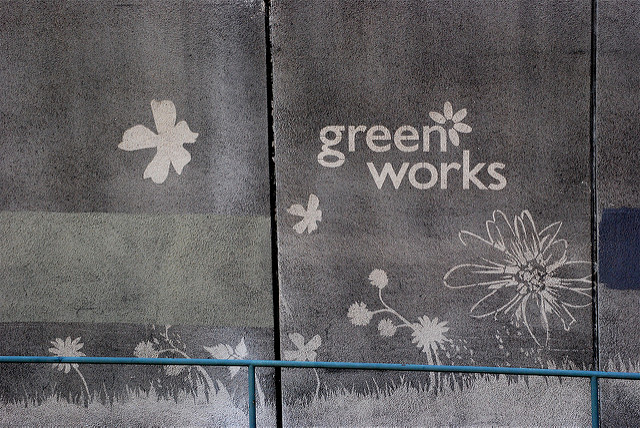
\includegraphics[width=55mm]{img/reverse-graffiti.jpg}
	\centering
	\caption{Reverse graffiti. \textcopyright  Lisa Müllerauh}
	\label{fig:defGrowthHacker}
\end{figure}

\begin{figure}[h!]
	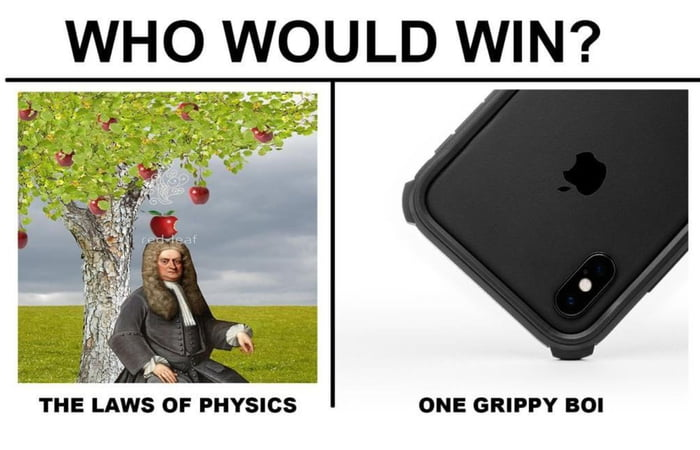
\includegraphics[width=\linewidth]{img/dbrand-internetmeme.jpg}
	\centering
	\caption{Internetmeme van dbrand. Ze spelen in op een recent memeformaat en passen het toe op hun eigen product(en). Zo kunnen ze met amper budget, enkel owned en earned media, een heel groot publiek laten weten dat hun product bestaat.}
	\label{fig:defGrowthHacker}
\end{figure}

\section{Wat is growth hacking?}
\label{sec:wat-is-growth-hacking}
Growth hacking is ook een nieuwe trend binnen marketing die vaak onduidelijkheid met zich mee brengt. Dus dan komt de vraag: wat is growth hacking nu exact?

Nicholas D’hondt beschrijft growth hacking in een artikel van~\textcite{Birdhouse2019} als een mindset van heel veel experimenteren en constant op zoek gaan naar nieuwe kanalen die kunnen zorgen voor groei. 

Het gaat om zoveel mogelijk mensen binnen je doelgroep te bereiken, zo kan je als bedrijf met (zeer) weinig geld een groot resultaat behalen. 

Sommige bedrijven willen een bepaalde boodschap verspreiden, andere willen enkel hun merknaam naar buiten krijgen. Het draait steeds om groeien, in welk specifiek gebied dat je wil groeien moet je voor ieder experiment steeds definiëren. Zo kan je leren uit het experiment, het is namelijk niet de bedoeling dat er zomaar uit het niets wordt geëxperimenteerd. Er zullen veel experimenten falen en het is de bedoeling dat er steeds iets uit geleerd kan worden. Dit is mogelijk door op voorhand goed te weten wat het doel is, ook moet er achteraf genoeg documentatie voorzien worden van het experiment. Waarom het doel al dan niet behaald werd kan veel verduidelijking geven en kan je in de juiste richting duwen.

Wanneer er kleine realistische (en S.M.A.R.T.) doelen gezet worden zorgt dit ook een goed mentaal effect, je komt in een soort "flow" terecht, veel momentum door het steeds behalen van de doelen. Dit zorgt voor veel motivatie en het creëert ruimte om te experimenteren. Het S.M.A.R.T. principe is een afkorting en staat voor:
\begin{itemize}
	\item Specifiek - Is de doelstelling eenduidig?
	\item Meetbaar - Onder welke (meetbare/observeerbare) voorwaarden of vorm is het doel bereikt?
	\item Acceptabel - Zijn deze doelen acceptabel voor de doelgroep en/of het management?
	\item Realistisch - Is het doel haalbaar?
	\item Tijdsgebonden - Wanneer (in de tijd) moet het doel bereikt zijn?
\end{itemize}

Bijvoorbeeld: ``Over vijf jaar wil ik projectmanager zijn, verantwoordelijk voor ICT-projecten van 100.000 tot 1.000.000 euro.`` \textcopyright carrieretijger.nl

In de podcast van ~\textcite{fizzle.co2015}~\citetitle{fizzle.co2015} wordt growth hacking aanzien als een buzzword, wat op dit moment zeker wel waar is. Ondanks dat de term buzzword wordt gebruikt, betekent dit niets slecht. Ze erkennen ook de mooie kanten van growth hacking zoals de creativiteit van growth hackers (of growth hacking teams). Ze worden verplicht om creatief te zijn, omdat er geen geld is. 

De slechte kant van growth hacking is volgens de podcast van~\autocite{fizzle.co2015} dat sommige mensen het zien als een manier om het systeem te "hacken", te misbruiken, om zo veel aandacht tot het product of bedrijf te krijgen. Dat is natuurlijk geen lange termijn strategie.

Een goed voorbeeld van growth hacking is het experimenteren van een schaalbare aanpak waarbij gebruikers zelf zorgen voor meer gebruikers. In een ideale situatie heb je zo'n goed product dat mensen er gek van zijn en dat deze ``viral factor`` ontstaat. Als men heel tevreden is van het product zal het zichzelf wel verspreiden. Groupon heeft het op deze manier aangepakt en is een goed voorbeeld hiervoor.

Opvallend is ook dat veel growth hacks een ``build-in expiration date`` hebben. Dat wil zeggen dat ze na een tijdje niet meer zullen werken. Een goed voorbeeld is Facebook advertenties: vroeger kon je dit gebruiken als growth hack. Je kon door je aanwezigheid op Facebook heel veel mensen binnen je doelgroep bereiken. Op dit moment wordt het niet meer gezien als growth hack, doordat de keywords waarop men wil adverteren te duur zijn geworden.

\begin{figure}[h!]
	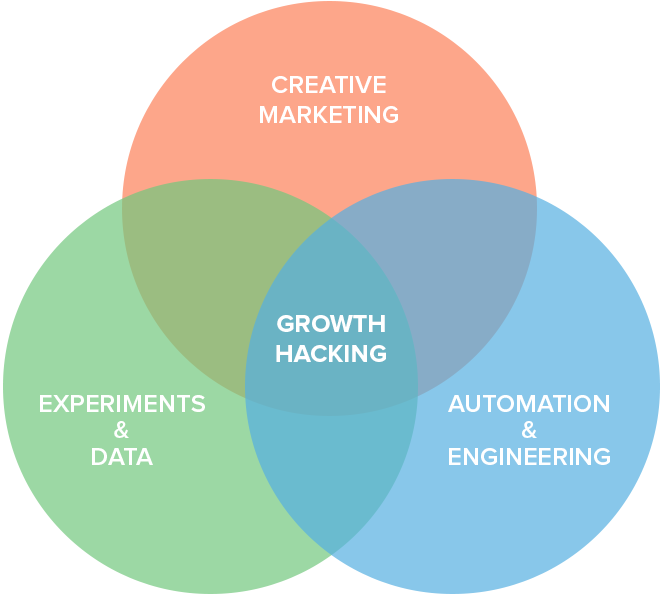
\includegraphics[width=\linewidth]{img/growth-hacking-essential-parts.png}
	\centering
	\caption{Essentiële onderdelen van growth hacking. Bron: \autocite{Rosado2018}}
	\label{fig:partsGrowthHacking}
\end{figure}

\subsection{Voorbeelden van growth hacks} \label{sec:growth-hacking-voorbeelden}
\begin{itemize}
	\item \textbf{Airbnb}: Gebruik maken van de community van Craigslist\footnote{Craigslist is een online platform dat voornamelijk in de Verenigde staten gebruikt wordt. Het wordt gebruikt om vacatures, woningen, cv's en dergelijke op te plaatsen.}. Airbnb stuurde e-mails naar de gebruikers van Craigslist die hun woning op dat platform geplaatst hadden met het verzoek om deze ook op Airbnb te plaatsen. Het werkte ook in de omgekeerde richting: vanuit Airbnb kon je met 1 klik je woning op Craigslist plaatsen (met een link terug naar Airbnb natuurlijk). 
	\item \textbf{Dropbox}: een referral programma\footnote{Wanneer je iemand doorverwijst naar de service of een product van een bedrijf en je hiervoor vergoed wordt.} dat voor beide partijen voordelig is. Wanneer men iemand succesvol kon laten registreren, via een persoonlijke link, kregen beide partijen gratis opslag op Dropbox.
	\item \textbf{Hotmail}: De eerste growth hack, ``PS: I Love You``. Onderaan iedere e-mail werd er één lijn toegevoegd: ``PS: I love you. Get your free e-mail at Hotmail.``. Waarbij Hotmail een link was naar de registratiepagina. 
	\item \textbf{Spotify}: Door de nauwe samenwerking met Facebook kon je steeds zien naar welke liedjes je vrienden luisterde op Spotify. Zo ontdekte duizenden mensen het platform en ze konden eenvoudig een account aanmaken door in te loggen via Facebook. Spotify gebruikt nu nog steeds growth hacks, zoals de verschillende partnerships met bedrijven zoals Facebook Messenger, Tinder, enz. Het is makkelijker dan ooit om een liedje door te sturen naar je vrienden, via Spotify.
\end{itemize}

\subsection{Growth hacking binnen een bedrijf} \label{sec:growth-hacker-functie}
Een growth hacker is half marketeer en half ingenieur, zoals vermeld in het onderzoeksvoorstel en geïllustreerd door de afbeelding hieronder.
\begin{figure}[h!]
	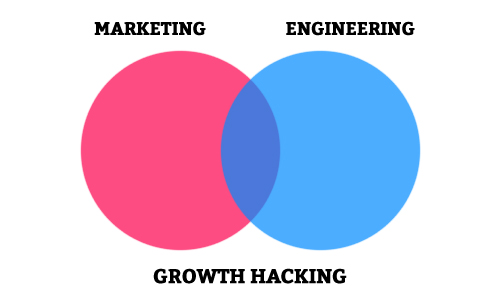
\includegraphics[width=\linewidth]{img/growth-hacker-definition.jpg}
	\centering
	\caption{Definitie van growth hacking, "Growth hacking as a fusion of two fields"  (Brody 2013, geciteerd 13.05.2016)}
	\label{fig:defGrowthHacker}
\end{figure}

In het artikel van The Birdhouse~\citetitle{Birdhouse2019} vertelt Nicholas dat growth hacking moet leven in de hele organisatie. Er moet een team gecreëerd worden met mensen uit verschillende branches van het bedrijf: developers, entrepreneurs, marketing en sales zetten we bij elkaar. In deze situatie is er niet één growth hacker, er kan wel iemand zijn die alle mensen bij elkaar brengt en het concept van growth hacking uitlegt. Als we die persoon als growth hacker zien is hij of zij eerder een soort coach die het team zal helpen om rond growth hacking te brainstormen.

Bij kleinere bedrijven kan het zijn dat er één growth hacker is, deze zal dan het profiel hebben van een marketeer en ingenieur en zal doorheen het bedrijf informatie moeten vergaren. Met al die informatie kan hij of zij experimenten bedenken of collega's aanspreken en hun ideeën implementeren of deze verwerken en doorgeven aan de developers of andere marketeers. 

In de podcast,~\citetitle{fizzle.co2015}, van~\autocite{fizzle.co2015} spreken ze over een ingenieur die aan marketing doet. Dat is het profiel van een growth hacker volgens hun. Ze zien het zo omdat een ingenieur vaak een ``data-driven`` aanpak heeft, denken vanuit data om zo experimenten in eerste instantie te creëren en vervolgens ook bij te sturen. 

Het is ook belangrijk om steeds feedback te vragen aan je collega's en natuurlijk ook de klanten, zo kan er samen aan het product gewerkt worden.

\section{Wat is het verschil met guerrillamarketing?} \label{sec:verschil-met-guerrillamarketing}

In~\citetitle{fizzle.co2015}~\autocite{fizzle.co2015} wordt er dieper ingegaan op het bredere concept van ``Zero Budget Marketing``. Ze praten over growth hacking als een tactiek binnen guerillamarketing. 

Guerillamarketing is eerder ``old-school`` en gaat ook breder dan growth hacking. Bij growth hacking ligt de focus op het digitale, dus online verschillende experimenten uitvoeren. Het is een hele nieuwe dimensie waarbij men dus eerder denkt aan growth hacking en niet guerillamarketing.

Zoals in \ref{subsec:guerrillamarketing} uitgelegd is guerillamarketing een marketingtechniek waarbij men vooral fysieke acties zal ondernemen om groei of naambekendheid te realiseren. 

\section{Hoe begin je aan growth hacking?} \label{sec:hoe-growth-hacking}
 
Zoals eerder vermeld draait growth hacking om de experimenten die je uitvoert, maar hoe begint men er aan?

Men kan eerst een audience (of groep mensen die je volgen) opbouwen, zoals @portland heeft gedaan op Instagram, en achteraf een bedrijf opstarten rond je bestaande audience, zoals @portlandgear. Het zijn 2 Instagram-accounts van dezelfde persoon, hij of zij zag dat er interesse was voor producten in verband met portland. Daardoor was het creëren van een webshop een zeer goed idee, toen was @portlandgear geboren. Via de eerste Instagram-account worden er posts gezet met producten van de tweede account.

Het is een voorbeeld van hoe je met growth hacking aan de slag kan. Natuurlijk lopen lang niet alle growth hacks op die manier. Het gaat ook helemaal niet heel snel of plots, je moet bijvoorbeeld in zo'n Instagram-account veel tijd steken en zorgen dat het interessant is om te volgen. Als dat niet het geval is gaat er niemand de account volgen en zijn er dus geen potentiële klanten.

Naast het Instagram voorbeeld zijn er enkele algemene regels waar men zich aan kan houden voor het opstellen van goede experimenten. 

\begin{itemize}
	\item Data is key: alles moet opgeslagen worden, dus alle tracking-tools moeten werken en getest zijn
	\item Zodra alles voldoende kan opgevolgd worden kan men beginnen denken over het doel van het eerste experiment. Het is belangrijk om een duidelijk, S.M.A.R.T. doel te hebben, zoals eerder vermeld.
	\item Dan begint men met het zoeken van de personas die men wil bereiken én waar deze te vinden zijn. Welke kanalen er best gebruikt kunnen worden om deze personas te vinden.
	\item Nadat het experiment is uitgevoerd kunnen er via de tracking-tools veel vragen beantwoord worden. Of het aantal bezoekers op de website al dan niet gestegen is, of de omzet gestegen is, wat het resultaat is op sociale media. Enzovoort... 
\end{itemize}

In het volgende hoofdstuk wordt er dieper ingegaan op hoe je growth hacking kan toepassen op een bedrijf. Dit wordt bevestigd door verschillende mensen in het werkveld, die geïnterviewd worden met gerichte vragen rond het onderwerp.


%%=============================================================================
%% Methodologie
%%=============================================================================

\chapter{Methodologie}
\label{ch:methodologie}

%% TODO: Hoe ben je te werk gegaan? Verdeel je onderzoek in grote fasen, en
%% licht in elke fase toe welke stappen je gevolgd hebt. Verantwoord waarom je
%% op deze manier te werk gegaan bent. Je moet kunnen aantonen dat je de best
%% mogelijke manier toegepast hebt om een antwoord te vinden op de
%% onderzoeksvraag.

- Interview met verschillende (4-6) start-ups
- Digital Marketing experts interviewen (Jaimy, RVI, ...)
- "Al gehoord van Growth hacking?", "Zijn jullie al op zoek geweest Growth hacks?", ...

\lipsum[21-25]


%%=============================================================================
%% Interviews
%%=============================================================================

\chapter{Interviews}
\label{ch:interviews}

De interviews worden in dit hoofdstuk uitgeschreven en op het einde van ieder interview wordt deze samengevat.

\section{Interview Filip Polfiet}
\label{sec:interview-filip}

Filip is een Digital Marketeer, of Migital Darketeer zoals hij zichzelf noemt, met 3 diploma's. Hij heeft eerst zijn diploma journalistiek behaald, daarna politieke en sociale wetenschappen en als laatste confict en development wat ontwikkelings samenwerking betekent. Na al deze diploma's en de vele jaren studeren heeft hij op zichzelf wat liggen omscholen naar de online webtechnologieën. Dit gaat van Wordpress websites tot de achterliggende architectuur en HTML, CSS, JS, ... en verder naar de SEO, SEA en het opvangen van alle data in Google Analytics en zoveel meer. Nu is Filip freelance consultant voor een digital agency en een start-up van de Belfius Bank. Voordien heeft Filip veel ervaring binnen het vak als digital marketeer, web master, community manager en copywriter. Ook heeft hij een goed inzicht in het creatieve deel van marketing zoals het maken van posters, filmpjes, geluidsbewerking en dergelijke.

\begin{itemize} 
	\item Heeft u al van growth hacking gehoord?
	
Ja. Het is vooral een creatieve marketing strategie die veel impact heeft met weinig budget. Denk aan guerrillamarketing. Jammer genoeg is het vaak geforceerd doordat andere bedrijven hetzelfde proberen als andere bedrijven maar dat werkt niet. Of toch meestal niet

	\item Zo ja: hoe past u dit toe binnen uw bedrijf?
	
Vb: Woody: vrij klassiek bedrijf dat geen super opvallende marketing nodig heeft. Het is natuurlijk ook iets dat niet enkel via Facebook Ads kan (wat Filip doet voor Woody als consultant vanuit het digital agency RVI media uit). Jammer genoeg is het ook iets dat veel bedrijven niet durven. Growth hacking is ook durven, dingen uitproberen, experimenteren en falen. Dat is wat meer (grote) bedrijven moeten durven.
	
	\item Zo nee: past u dit concept toe op een andere manier binnen het bedrijf waar u voor werkt?
	
/

	\item Wat zijn uw belangrijkste resources voor de groei van een bedrijf? Steunt u op AdWords, Facebook Ads etc?
	
Groei is een en-en-verhaal. Je moet meerdere kanalen gebruiken zoals E-mail, Facebook Ads, Instagram Ads (via het FB ads platform), Google ads (wat minder belangrijk is omdat niet per sé creatief is, het werkt eerder ondersteunend). FB ads is een goede tool omdat onderzoek doet blijken dat de gemiddelde belg of europeaan minstens 30 min per dag aan zijn GSM besteed.

	
	\item Hoe ging u in het begin van uw carrière om met (community)-groei van een bedrijf en hoe doet u dat nu? Wat is er veranderd in die tijd? Wat heeft u geleerd?
	
Toen Filip begon bestond er geen Social Media en al zeker geen social media advertisements. De websites bestonden nog maar net en waren geen "big deal". 
Nu is er social media en talloze websites. Men kan spreken van een information overload. Het heeft enorm veel voordelen in verband met marketing zoals de toegang tot meerdere kanalen (Social media, e-mail, ...) en dat het heel meetbaar is.
		
	\item Heeft u ervaring met Zero Budget Marketing? Wat is hierbij het belangrijkste onderdeel van marketing?
	
	Het belangrijkste is om heel creatief te zijn. Je moet alle kanalen gebruiken die beschikbaar zijn. Je moet je verspreiden via al die kanalen, en zo'n dingen zijn zeer moeilijk met weinig budget, maar zeker mogelijk, mits goede brainstorm sessies en een goed idee. 
	
	Uit eigen ervaring bij Plan België: op Pukkelpop wou Plan België een actie doen rond kind huwelijken. Initieel wouden ze flyers uitdelen op het festival, maar Filip wou dit origineler aanpakken. Het moet verder gaan dan enkel flyers uitdelen, daarmee bereik je niet veel bij de doelgroep van 15-25 jarigen. Dus Filip bedacht het idee van een stand waar koppels of vrienden zichzelf konden "uithuwelijken". Hier konden ze een ludieke foto nemen en tijdens het proces of achteraf kregen ze een uitleg dat deze leuke stand eigenlijk wel meer betekenis had dan enkel een toffe foto maken met je vrienden. Er zat veel meer achter en bracht zo aandacht bij de jongeren dat er in vele landen wel effectief een probleem is dat jonge meisjes worden uitgehuwelijkt aan een oudere man waar ze helemaal niet mee willen samen zijn. Filip heeft hierbij de volledige uitwerking verzorgd, van idee tot uitwerking van de stand en bijstand van het IT-team. Want dit maakt het zero budget marketing idee ook wel growth hack, doordat IT, marketing en creatieve ontwerpers samenkomen. Aan deze stand was een hele technische kant verbonden waarbij je je e-mailadres kon invullen en wanneer je dan een foto nam kreeg je die foto opgestuurd naar je e-mailadres. Ook was er een iPad voorzien waarmee je een foto kon nemen en deze eenvoudig uploaden op je social media.
	
	Een tweede ervaring, ook bij Plan België, ging over een simpele social media post dat inspeelde op een in die tijd populaire trend: ``Keep calm and ****``. Filip speelde hier op in tijdens moederdag, waar hij de briefing kreeg om een leuke post te maken voor sociale media in verband met sociale media en moederdag. Hij schreef een eenvoudige post met ``Keep calm and don't forget moederkesdag``. Enkel de manier waarop ``moederkersdag`` werd geschreven zorgde voor verschillende reacties en mensen die reageerde op deze post, elkaar tagde enz... Dit toont aan hoe belangrijke de juiste copywriting is en een combinatie van een originele post die inspeelt op de huidige trends.
	
	Een derde ervaring bij Plan België is een groot IT project waarbij ze een eigen crowd funding platform hebben kunnen starten voor vrij weinig geld, ongeveer 25.000 euro. Hier kon iedereen een eigen project starten met een foto en wat tekst waarbij ze hun reden voor geldinzameling verkondigden. Dit kan bijvoorbeeld een huwelijksjubileum zijn, waar de twee getrouwde geen cadeaus willen, maar enkel een goed doel steunen. Dat kan dan via het online platform waar ze enkel een link moeten delen. Daardoor moet het niet meer via hun eigen bankrekening gebeuren. Deze link kan ook verder op sociale media gedeeld worden en zorgt dus voor het belangrijke onderdeel van marketing: referral.
	
	Het laatste voorbeeld is bij Woody, het pyjama bedrijf in Gent: je moet steeds de realiteit en actualiteit in het oog houden. Je moet als marketeer heel bewust zijn van de feiten en deze in iets positief kunnen omzetten. Bijvoorbeeld: de website van Woody lag tijdens de Sint-periode plat, door een technisch probleem. Als digital marketeer kan je hier heel leuk mee omgaan, zoals Filip deed, met een ludieke post. Filip heet een foto van de sint die iemand voor Woody had gemaakt, bewerkt met een draad, waar de sint over viel. Hierbij werd te tekst geplaatst "De sint struikelde over de draad en heeft perongeluk de website neergehaald, we doen ons best om dit op te lossen!". Door deze leuke post is iedereen op de hoogte en toch niet boos op het bedrijf.
	
	\item Waaruit bestaat een ideaal marketing team volgens u? In verhouding: hoeveel copywriters, digital marketeers, programmeurs, creatief ontwerpers, enz.?
	
	De basis is volgens Filip sowieso: een copywriter, grafisch ontwerper en een programmeur/analytisch denker dit met de cijfers en de code kan werken. Hierbij hoort steeds ook een out-of-the-box denker of een gek persoon. Deze kan 1 van de andere functies delen, zoals copywriter.	
	
	Verschillende personen zijn belangrijk, natuurlijk is dit afhankelijk van de grootte van het bedrijf. Er mag geen negatief persoon tussen zitten die niet open staat voor andere ideeën tijdens de brainstorm sessie, want zo creëer je een negatieve sfeer. Je mag tijdens zo'n sessies niet te realistisch zijn; ``dit kan niet want x en y`` is niet wat je wil. Je kan moeilijk op een goed, creatief idee komen in een vergadering met 20 mensen waarvan enkele accountancy en managers dit te veel met cijfers bezig zijn. Je moet los van de cijfers, los van het budget kunnen ``freewheelen`` en het volledige tegenovergestelde durven denken dan dat wat er gepland is. Dit kan moeilijk om een voorafgedefinïeerde tijdspanne, zoals 4 uur in de namiddag. Zo'n ideeën hebben tijd nodig.
	
	\item Hoe belangrijk is viraal gaan voor een bedrijf? Is dit volgens u waar iedere marketeer, zoals uzelf, naar streeft? Of is het een specifiek doel dat op de juiste moment wordt achtervolgd?
	
Dit gaat natuurlijk niet altijd en is iets dat moeilijk is. Het kan bijvoorbeeld 1 keer per jaar, maar het is niet iets dat consistent kan gebeuren. De post op sociale media moet bijvoorbeeld heel creatief, goed gevonden en origineel zijn voordat deze viraal kan gaan. De creativiteit staat centraal hierbij. Natuurlijk hopen veel digital marketeers dat hun post viraal gaat, maar dit is natuurlijk zelden het geval. Bedrijven moeten hier ook niet op focussen, goede content is beter dan geforceerde content die bedoeld is om viraal te gaan.

Een virale post kan van alles zijn en is vaak toevallig. Het kan een goed getimede gif zijn van een sociale media community manager of een leuke reactie op Twitter of een goede post die op de juiste moment is gepost in de juiste context, ... Soms lijken deze reacties of posts heel spontaan, maar is er door de bedrijven wel goed over nagedacht.
	
	\item Bij growth hacking spreekt men vaak over 2 à 3 belangrijke onderdelen: Creativiteit, Experimenteren/Analyseren van data en tot slot het Automatiseren en toepassen op technisch vlak. Ook bent u niet bewust bezig met growth hacking, deze onderdelen komen ook aan bod bij traditionele of digitale marketing.
	\begin{enumerate}[label*=\arabic*.]
		\item Creativiteit: Hoe gaat u om met het creatieve proces van marketing? Bijvoorbeeld: Zijn hier brainstorm sessies voorzien? Heeft u creatieve ontwerpers die helpen?
		
		Volgens Filip is het de basis van alles. Je moet eerst veel nadenken voordat je begint met ontwikkeling van het technische aspect van je idee. De start is steeds een goed en creatief idee. Het is belangrijk om hier voldoende tijd aan te spenderen voordat je verder gaat.
		
		\item Data: Welke tools gebruikt u om informatie te verzamelen over uw doelpubliek? Welke tool is het belangrijkst en waarom?
		
		Google Analytics
		
		\item Automatiseren: Welke rol speelt IT of het IT-team bij marketing volgens u? 
		
		Het IT team speelt een heel belangrijke rol, maar daar loopt het vaak fout. De communicatie en vlotte werking is cruciaal, het is vaak moeilijk om iets gedaan te krijgen in een IT team. Hiervoor is goede communicatie belangrijk.
		
		De laatste 2 punten, Data en automatiseren zijn bijkomend en eerder logisch, terwijl het eerste punt, de creativiteit het belangrijkste en moeilijkste proces is van de 3.
		
	\end{enumerate}
	\item In de termen van growth hacking: is er een experiment dat u al lang wil uitvoeren, maar nog geen middelen heeft voor gehad?
	
	Een nieuw concept, een eigen start-up waar alles mogelijk is. Niet per sé iets heel concreet, maar een bedrijf waar men durft risico's nemen, want het risico is klein, want het kost niet veel.
	
	\item Growth hacking is vooral gekend bij online start-ups zoals Airbnb, Hotmail en Dropbox. Veranderd er volgens u veel bij growth hacking wanneer het niet meer gaat om een online bedrijf, maar wel een start-up met een fysiek product, zoals de krekelreep van Kriket?
	
	Het is zeker mogelijk, want het is een nieuw, origineel en creatief product. Het belangrijkste wordt een originele invalshoek vinden. Voor Kriket is het belangrijk om in te spelen op de actualiteit, zoals het klimaat. Ze moeten zoeken naar wie er geïnteresseerd is in een Kriket-bar. Wie durft zo'n krekelreep op te eten? Dat moeten ze uitzoeken. Een voorbeeld kan zijn; de ``Kriket challenge``. Hier kan men inspelen op de brug dat de meeste belgen maken van nog nooit insecten gegeten te hebben naar een Kriket-bar. Na de krekelreep is het ijs vaak gebroken en durft men andere insect-gebaseerde gerechten te eten. Rond het concept van de challenge kunnen enkele leuke video's gemaakt worden die in een marketing campagne gebruikt kunnen worden. De video's kunnen de extreme emoties weergeven die mensen hebben bij hun eerste bijt van een krekelreep met achteraf de brede glimlach waaruit blijkt dat het echt lekker is. En dat met geen schrik moest hebben voor de krekels in de krekelreep. ``Durft gij het aan?`` zou een mogelijke manier zijn om de campagne te nemen. Waar willekeurige mensen worden uitgedaagd om de krekelreep te proberen.
	
	\item Wat denk je van growth hacking? 
	
	Goed als klein bedrijf dat zoekt naar snelle groei. Het houdt in dat je veel risico neemt en heel creatief bent met je campagne of growth hack.
	
\end{itemize}


\section{Interview Damien Querbes}
\label{sec:interview-damien}

De technische data analytics, IT kant

Damien Querbes, opgegroeid in Parijs, heeft 2 masters behaald, in ``Corporate Finance`` en ``Entrepreneurship``. Na deze studies heeft hij 3 stages gedaan bij verschillende bedrijven. Bij zijn eerste stage lag de focus op financiën, de tweede stage was eerder ondernemen en de laatste stage was in een start-up. 

Tijdens die laatste stage is Damien geheadhunt en werd hij de rechterhand van 2 co-founders van Europecar en Ubeeqo. De 2 bedrijven werden toen samengevoegd, dus ook de teams en de bedrijfsculturen. Hij heeft veel gewerkt in Brussel, Parijs en Berlijn, in het laatst vermelde land heeft hij een opleiding gekregen van een collega, die nu nog steeds een goede vriend is van hem. Zijn collega heeft hem opgeleid in digital marketing en toen heeft hij de smaak van marketing te pakken gekregen. Hij heeft geholpen met een nieuw merk te gaan rebranden. Een bedrijf van B2B naar B2C omzetten, prijzen bepalen en andere strategische beslissingen nemen.

Naast deze enorme opgave begon Damien meer en meer interesse te krijgen in digitale marketing en vooral de data die er allemaal bij komt kijken. Daarom is hij beginnen leren programmeren, zo kon hij nauw in contact staan met het IT team en het proces begrijpen waar ze door gaan. Hij kreeg de titel ``Marketing Architect``, waarbij het hele IT-deel van het marketing-team moest managen. De infrastructuur van alle tools die gebruikt worden tot de heel technische samenwerking tussen deze tools.

Nu heeft hij besloten om een nieuwe uitdaging aan te gaan bij Jaimy, als Head of Marketing probeert hij het online platform Jaimy aan de man te brengen.

\begin{itemize} 
	\item Heeft u al van growth hacking gehoord? Zo ja: hoe past u dit toe binnen uw bedrijf?
	
Ja, Damien kent growth hacking via zijn carrière die hij heeft opgebouwd. Hij heeft de term growth hacking zien groeien, de hype zien stijgen en begrijpt het concept dus goed.

Hij gebruikt het niet, hij gelooft niet in Growth hacking. Het is een short-term strategie. Damien verkiest een long-term strategie waarbij je uiteindelijk meer bereikt. Desondanks zijn er wel enkele growth hacks die hij gebruikt en aanraadt, maar dit betekend niet dat hij growth hacking een goede marketingstrategie vindt op zich. 

De growth hack die Damien recent heeft toegepast is het toevoegen van ``?location=Brussel`` aan de link vanuit de advertenties. In de Google en Facebook advertentie platformen kan je dynamisch de stad toevoegen. Met deze link voelt de website veel persoonlijker aan en uit de cijfers is er bewijs dat dit de conversies verhoogd.

\begin{figure}[h!]
	
\includegraphics[width=\linewidth]{img/location-growth-hack.png}
	\centering
	\caption{De simpele growth hack die Damien heeft toegepast op de website van Jaimy (\href{https://jaimy.be/nl/?location=Brussel}{https://jaimy.be/nl/?location=Brussel})}
	\label{fig:fantalism}
\end{figure}
	
	\item Wat zijn uw belangrijkste resources voor de groei van een bedrijf? Steunt u op AdWords, Facebook Ads etc?
	
Aanvullende op de vorige vraag, goede long-term strategie die Damien nu toepast op Jaimy is het bouwen van de fundamenten van je merk. Dit doet hij via Google Adwords en Facebook Ads en hij baseert zijn advertenties op de basisdocumenten die bij de opstart van Jaimy zijn gemaakt. Dit zijn de missie, de visie, de USP's (Unique Selling Propositions); de meerwaarden dat de klanten uit Jaimy kunnen halen, het brandbook of huisstijlregelmentenboek (met de huisstijl, slogan, tone of voice, enz...) en de elevator pitch. 

Na het pushen van veel advertenties is het doel om de marketing langzaam aan over te laten gaan naar mond tot mond reclame. Dan zal er minder marketing aan deze kanalen gespendeerd worden. 

	\item Heeft u ervaring met Zero Budget Marketing? Wat is hierbij het belangrijkste onderdeel van marketing?
	
Heel moeilijk, je product moet heel uniek zijn
	
	\item Hoe ging u in het begin van uw carrière om met (community)-groei van een bedrijf en hoe doet u dat nu? Wat is er veranderd in die tijd? Wat heeft u geleerd?
	

	
	\item Waaruit bestaat een ideaal marketing team volgens u? In verhouding: hoeveel copywriters, digital marketeers, programmeurs, creatief ontwerpers, enz.?
	
	
	
	\item Hoe belangrijk is viraal gaan voor een bedrijf? Is dit volgens u waar iedere marketeer, zoals uzelf, naar streeft? Of is het een specifiek doel dat op de juiste moment wordt achtervolgd?
	
	
	
	\item Bij growth hacking spreekt men vaak over 2 à 3 belangrijke onderdelen: Creativiteit, Experimenteren/Analyseren van data en tot slot het Automatiseren en toepassen op technisch vlak. Ook bent u niet bewust bezig met growth hacking, deze onderdelen komen ook aan bod bij traditionele of digitale marketing.
	\begin{enumerate}[label*=\arabic*.]
		\item Creativiteit: Hoe gaat u om met het creatieve proces van marketing? Bijvoorbeeld: Zijn hier brainstorm sessies voorzien? Heeft u creatieve ontwerpers die helpen?
		
		
		
		\item Data: Welke tools gebruikt u om informatie te verzamelen over uw doelpubliek? Welke tool is het belangrijkst en waarom?
		
		
		
		\item Automatiseren: Welke rol speelt IT of het IT-team bij marketing volgens u? 
		
		
		
	\end{enumerate}
	\item In de termen van growth hacking: is er een experiment dat u al lang wil uitvoeren, maar nog geen middelen heeft voor gehad?
	
	
	
	\item Growth hacking is vooral gekend bij online start-ups zoals Airbnb, Hotmail en Dropbox. Veranderd er volgens u veel bij growth hacking wanneer het niet meer gaat om een online bedrijf, maar wel een start-up met een fysiek product, zoals de krekelreep van Kriket?
	
	
	
\end{itemize}


\section{Interview Thomas hugo}
\label{sec:interview-thomas-hugo}

Thomas hugo\footnote{Dit is geen typo: hugo wordt geschreven met een kleine ``h``. } heeft zijn eigen bedrijf, Arnesson Art (\href{https://arnesson.art/}{https://arnesson.art}) en werkt voert opdrachten uit voor andere als concept artist. Grafische vormgeving gestudeerd aan Sint Lukas te Brussel, daarna BAS te Mechelen. Daarna bij Demonstr8 gewerkt, die uitsluitend creatieve offline campagnes uitvoeren. Hij heeft gewerkt voor de grootste bedrijven in de sector zoals Coca-cola, ABInBev, Mars, enz.

\begin{itemize} 
	\item Heeft u al van growth hacking gehoord?
	
Geleerd op BAS, Belgian Art School, maar jammer genoeg niet op Sint Lukas (of het huidige Luca School of Arts). 
	
	\item Zo ja: hoe past u dit toe binnen uw bedrijf?
	
	Minder relevant, voor zijn freelance werk gebruikt Thomas het online platform Reddit. Specifiek de subreddit, een online forum op Reddit, ``/r/gameDevClassifieds``. Dit is een medium dat werkt voor hem, als freelancer, maar dat is iets dat een bedrijf veel moeilijker kan gebruiken. Thomas gebruikt Reddit op professioneel vlak op 2 manieren. 
	
	\begin{itemize} 
		\item Voor zijn eigen bedrijf gebruikt hij Reddit om opdrachten binnen te halen. Dit is heel direct en heel professioneel. ``Bezoek is mijn portfolio, kijk of ik nuttig kan zijn voor uw bedrijf of project, want ik zoek opdrachten``.
		\item Voor Fantalism\footnote{Fantalism (\href{https://fantalism.com/}{fantalism.com}) is de webcomic van Thomas hugo, die vroeger ``Jeff and George`` heette.} is dit volledig anders, daar is Fantalism het product. Het doel is om de webcomic populair te maken zodat hij meer sponsors kan halen voor zijn Patreon, want alleen dan wordt het winstgevend om er aan te werken. Voorlopig is dit vooral omdat hij het heel graag doet en om een duidelijk portfolio op te bouwen in de richting waar hij naartoe wil. Natuurlijk kan hij zijn nieuwe hoofdstukken niet steeds overal spammen, want dat werkt gewoon niet. Daarom gaat Thomas heel voorzichtig te werk en wanneer hij bijvoorbeeld een hoofdstuk heeft dat gaat over ``Dungeons and Dragons``, kan hij dit in een subreddit zetten die gaat over dit onderwerp. Zo hebben de mensen die het zien passeren mogelijk wel interesse in het hoofdstuk.
	\end{itemize} 
	\begin{figure}[h!]
		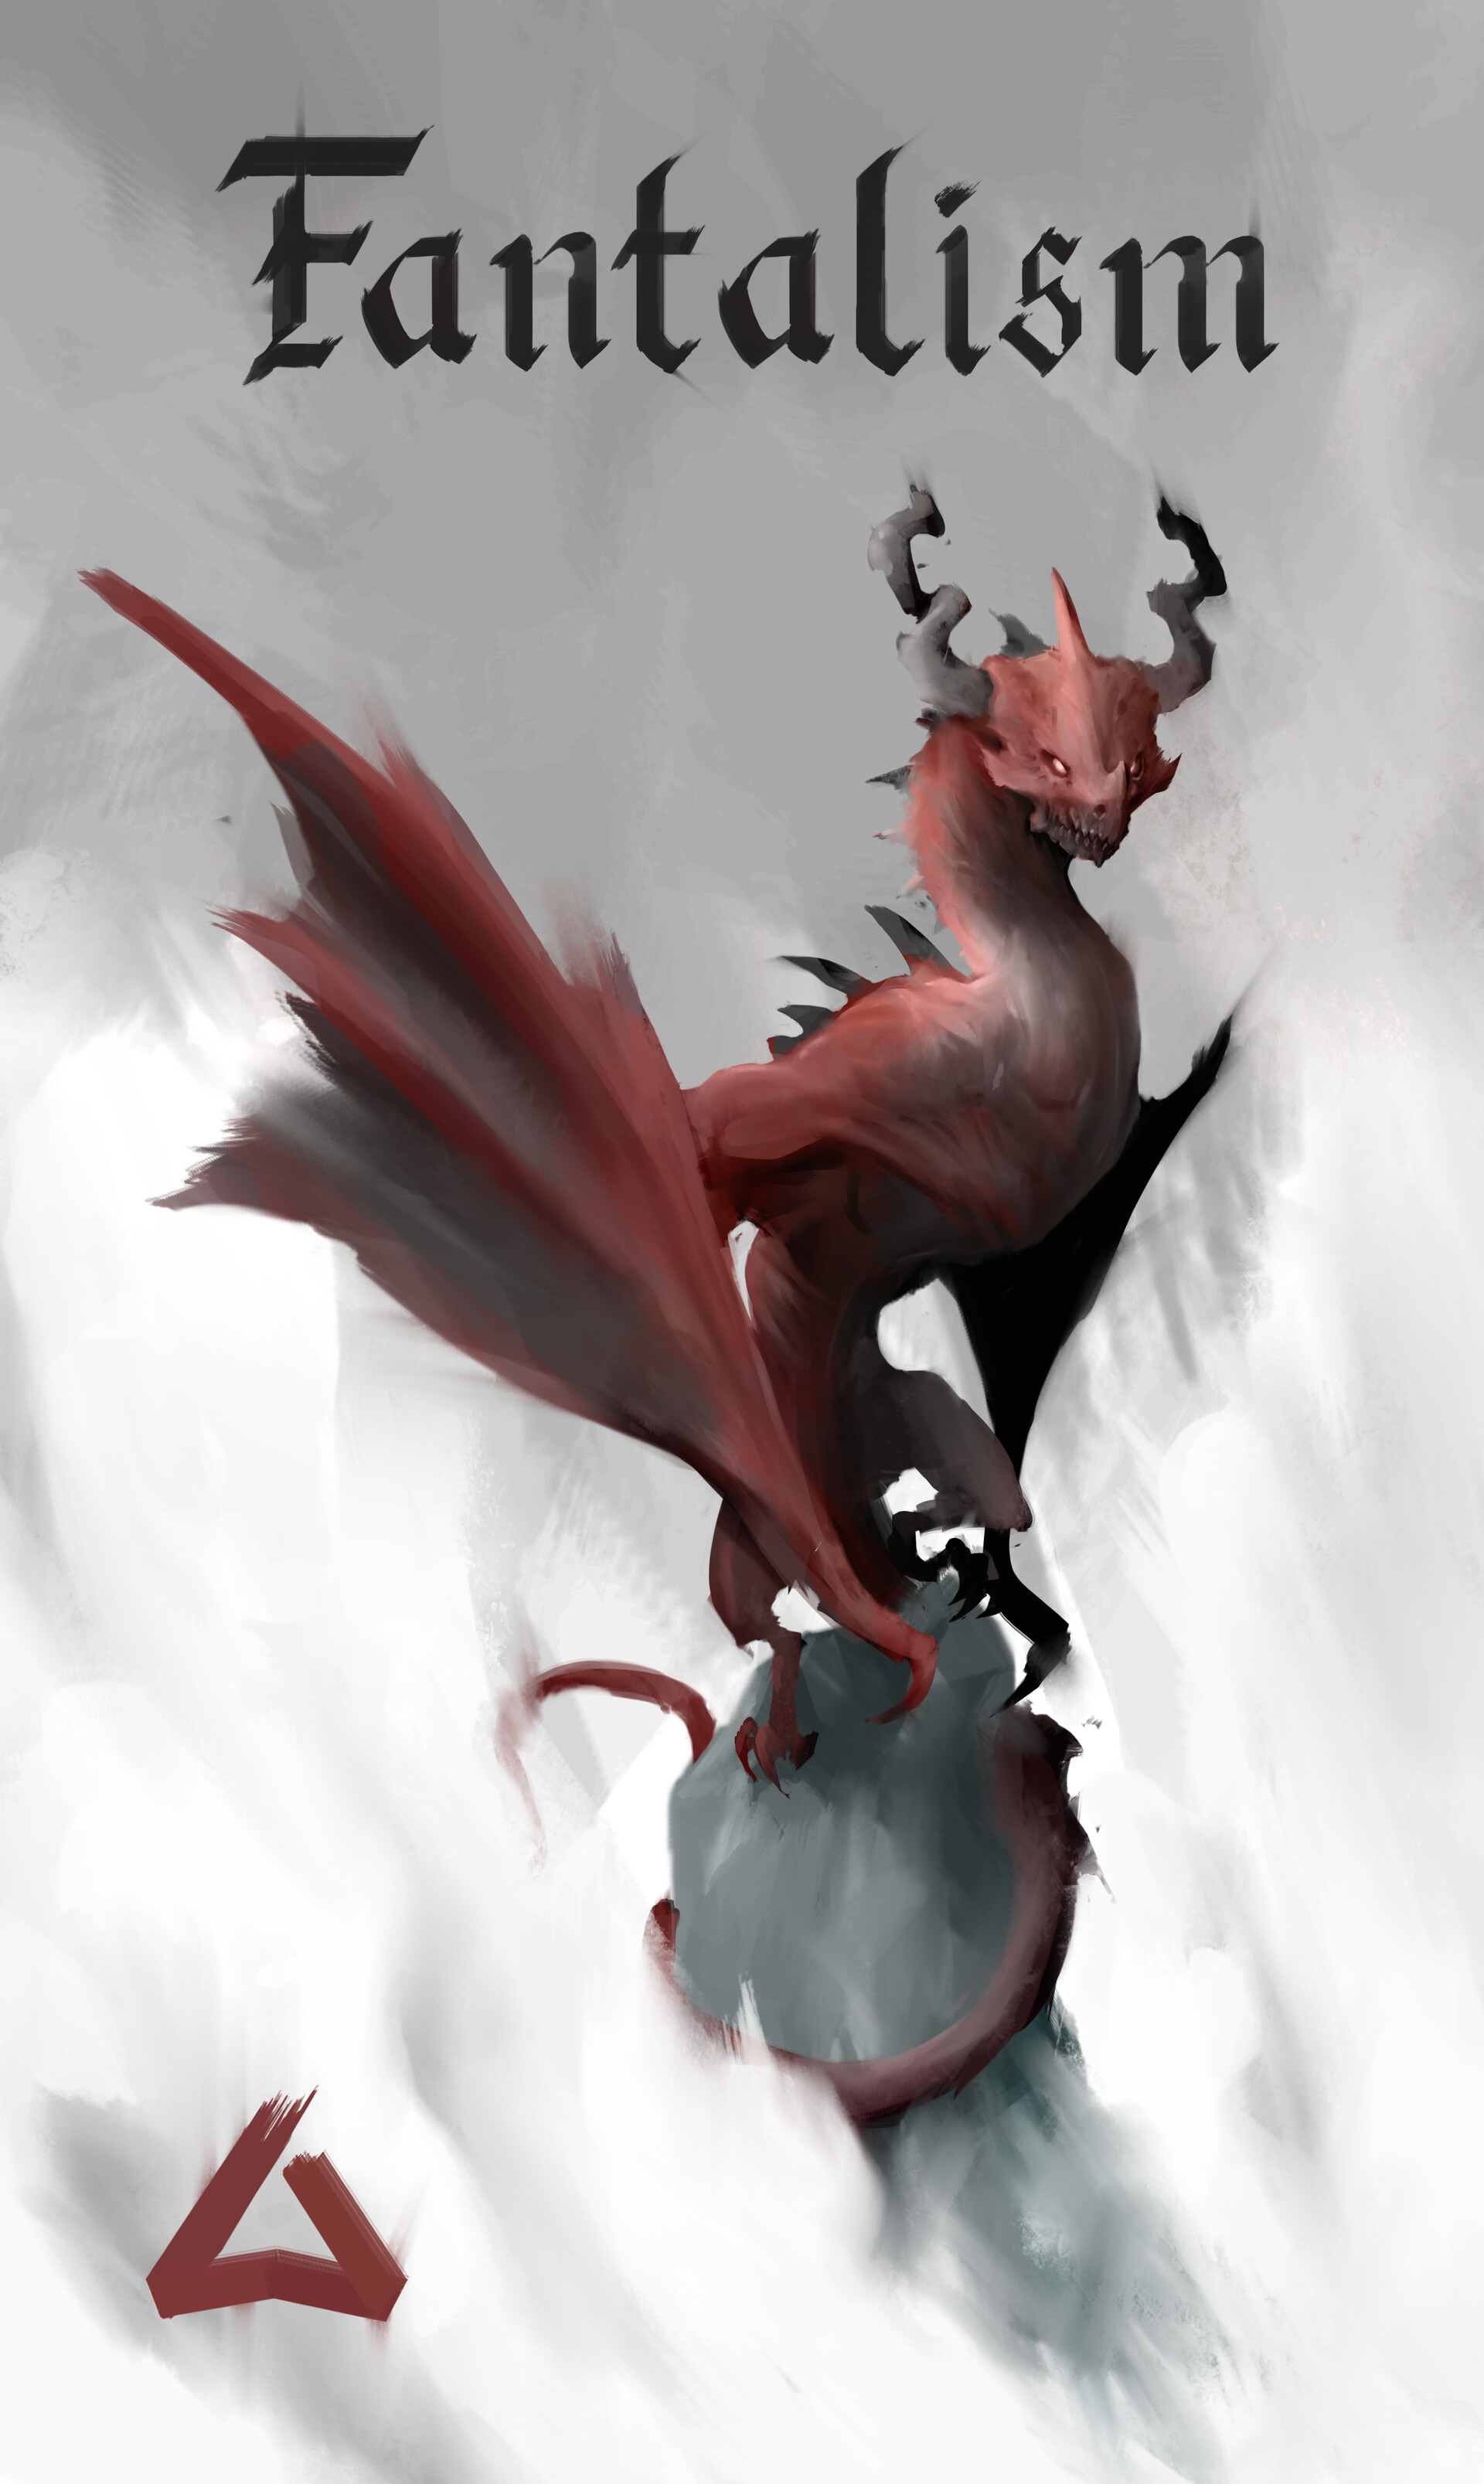
\includegraphics[width=50mm,scale=0.5]{img/arnesson-art-fantalism.jpg}
		\centering
		\caption{Fantalism: de webcomic van Arnesson Art, Thomas hugo.}
		\label{fig:fantalism}
	\end{figure}
	Thomas vertelde dat hij Reddit niet ziet als een ideaal medium voor te groeien. Het is als bedrijf moeilijk om deze kanalen goed te gebruiken. Als freelancer of gemotiveerde artist is dit veel toegankelijker, men wordt beter ontvangen op het platform.
	
	\item Wat zijn uw belangrijkste resources voor de groei van een bedrijf? Steunt u op AdWords, Facebook Ads etc?
	
	Voor Fantalism heeft Thomas Facebook Ads geprobeerd voor enkele tientallen euro's. Voor Thomas werkte dit echter niet zo goed, de interacties (lees: likes) die hij kreeg waren nutteloos. Ze deden dit enkel voor één post en hadden daarna geen interacties met nieuwe posts. Het was voor hem dus niet de moeite waard en het bleek dus moeilijk om op die basis een community uit te bouwen. Vandaar dat hij de aanpak behoudt van het posten op de juiste plaatsen, waar mensen interesse zouden tonen omdat ze het onderwerp heel leuk vinden. Die interacties zijn veel meer waard.
	
	Thomas ziet dit voor Kriket ook niet direct als dé manier. Hij stelt voor om gratis samples uit te delen op plaatsen waar de doelgroep van Kriket zit, zoals campussen van hoge scholen of universiteiten. Mensen die bewust zijn van de milieuproblematiek, die openstaan voor iets nieuws en die bezig zijn met hun gezondheid.
	
	
	\item Heeft u ervaring met Zero Budget Marketing? Wat is hierbij het belangrijkste onderdeel van marketing?
	
	Tijdens Thomas zijn opleiding in Sint Lukas werden er enkele keren opdrachten gegeven omtrent marketing. Toen gaven de docenten de opdracht om het met zo weinig mogelijk budget (zero budget marketing) te doen. Dit was dus nooit of zelden het geval, vaak kwamen medestudenten af met ideeën uit guerillamarketing, zoals flyers uitdelen. Maar dan werd er niet gedacht aan ``Wie gaan die flyers uitdelen?``, het antwoord was dan ``Studenten?``, ``En wie gaat die betalen?`` enzovoort... Het blijkt dus dat zero budget marketing zéér moeilijk is. Als je echt met geen of amper budget veel mensen wil bereiken moet je viraal gaan en dat is een grote uitdaging.
	
	\item Hoe ging u in het begin van uw carrière om met (community)-groei van een bedrijf en hoe doet u dat nu? Wat is er veranderd in die tijd? Wat heeft u geleerd?
	
	Thomas heeft voor zijn eigen bedrijf, Arnesson Art, ook moeten nadenken over groei. In eerste instantie was dit ``Hoe krijg ik opdrachten binnen?``. Zoals eerder vermeld heeft Thomas dit gedaan via Reddit. Hij heeft hieruit geleerd dat de directe aanpak goed werkt;
	
	\begin{itemize} 
		\item ``Ik ben beschikbaar voor opdrachten``
		\item ``Hier is mijn portfolio``
		\item ``Ik werk enkel tegen betaling``
	\end{itemize} 
	
	Die laatste is verrassend belangrijk, liet Thomas weten. Veel mensen verwachten vrijwilligerswerk of het delen van winst met een slecht idee, maar zo'n dingen betalen de huur van zijn appartement natuurlijk niet.
	
	Toen werd er gevraagd ``Je vertelde eerder dat je niet geloofde in zero budget marketing en dat dit bijna altijd meer geld kost dan men verwacht, maar dit is toch zero budget marketing?``. Hierop antwoordde Thomas dat het niet gratis is, het kost nog steeds veel tijd om zo'n goede concrete, duidelijke en aantrekkelijke post te maken. Voordat deze op de juiste subreddit wordt gezet, wordt er veel tijd in gestoken om ze goed te maken. Deze tijd zou anders gebruikt kunnen worden om een opdracht uit te werken. ``Time is money``, ervaart hij zeer sterk sinds hij freelancer is.
	
	\item Waaruit bestaat een ideaal marketing team volgens u? In verhouding: hoeveel copywriters, digital marketeers, programmeurs, creatief ontwerpers, enz.?
	
	Een goed marketingteam opstellen is een hele grote klus volgens Thomas. Alle kwaliteiten dienen samen te komen uit verschillende functies, dit wil zeggen:
	
	\begin{itemize} 
		\item Strateeg
		\item Copywriter
		\item Social media manager
		\item Creatief ontwerper
		\item Digital marketeer
		\item Programmeur of performance marketeer
	\end{itemize} 
	
	In een start-up zoals Kriket is het belangrijk dat het team zich verbonden voelt met het product. Het is bijna noodzakelijk dat je een passie hebt voor het product dat geproduceerd wordt.
	
	Volgens Thomas kan het voor Kriket kan het goed zijn om een nauwe samenwerking te starten start-up digitaal marketingbureau, waar het bedrijf gemotiveerd is om samen met Kriket te groeien. De communicatie met die bureau is dan zeker belangrijk, dus hier moet zorgvuldig iemand voor worden aangesteld.
	
	\item Hoe belangrijk is viraal gaan voor een bedrijf? Is dit volgens u waar iedere marketeer, zoals uzelf, naar streeft? Of is het een specifiek doel dat op de juiste moment wordt achtervolgd?
	
	Waarschijnlijk streven veel marketeers naar een virale post op sociale media, maar dit is niet altijd wat de klant wil. Wanneer de klant bijvoorbeeld 5000 verkopen wil realiseren, kan het zijn dat een virale post voor maar 300 verkopen kan zorgen. Viraal betekent niet per sé goed, dit is wat veel mensen fout begrijpen. Wanneer de doelgroep niet juist zit heeft en video met 50 miljoen weergaven geen meerwaarde voor het bedrijf tegenover een video met 5000 weergaven.
	
	Een goed voorbeeld hiervan is de video van Telenet die de nieuwe zender TNT had gelanceerd: ``Push to add drama``. Die video heeft nu meer dan 56 miljoen weergaven op TNT. Ondanks deze virale video heeft de zender TNT het maar ongeveer 1 jaar volgehouden. De video werd overal gedeeld, ook in het buitenland, maar daar heeft de zender helemaal geen baat bij. Met dit voorbeeld kan je vaststellen dat viraliteit absoluut geen garantie is voor succes.
	
	Wat je wél wilt is mond tot mond reclame creëren, waar men tegen elkaar enthousiast over het product verteld.
	
	\item Bij growth hacking spreekt men vaak over 2 à 3 belangrijke onderdelen: Creativiteit, Experimenteren/Analyseren van data en tot slot het Automatiseren en toepassen op technisch vlak. Ook bent u niet bewust bezig met growth hacking, deze onderdelen komen ook aan bod bij traditionele of digitale marketing.
	\begin{enumerate}[label*=\arabic*.]
		\item Creativiteit: Hoe gaat u om met het creatieve proces van marketing? Bijvoorbeeld: Zijn hier brainstorm sessies voorzien? Heeft u creatieve ontwerpers die helpen?
		
		Ten eerste is niet alle marketing creatief, dus het creatieve proces kan heel eenvoudig of onbestaande zijn. Bij dit soort marketing is het belangrijkste een goed design, de copy\footnote{De term ``copy`` wordt vaak gebruikt in deze branche om de tekst aan te duiden die (vaak) door een copywriter is geschreven.} is niet per sé creatief en kan eventueel gekopieerd worden van vroeger. Een goed voorbeeld is de solden periode, er zijn studies geweest over welke afbeelding en welke copy er werkt, dus die gebruiken de (grote) bedrijven. De bedoeling is dan gewoon om deze campagnes zo hard te pushen en te verspreiden dat iedereen ze gezien heeft, ze moeten helemaal niet creatief zijn.
		
		``Maar wat is dan wél creatieve marketing?```, dat is enerzijds een goede boodschap (copy) en een mooi en duidelijk beeld. Anderzijds is dit een goede strategische aanpak, bijvoorbeeld een partnership of een originele actie die er aan gekoppeld is.
		
		Een voorbeeld dat Thomas aanhaalde voor Kriket was als eerste een mooi beeld. Bijvoorbeeld een witte kast met een groene plant bovenop, met bladeren en stengels die naar beneden hangen. De kast ligt vol met Kriket bars die duidelijk gepresenteerd worden. Rond de kast zijn er veel echte krekels voor het kleine ``shock``-effect. Aan de hand van een spel dat via een mobiele applicatie of de Kriket website kan er een spel gespeeld worden, waar de winnaar gratis Krikets voor een aantal maanden krijgt.
		
		\item Data: Welke tools gebruikt u om informatie te verzamelen over uw doelpubliek? Welke tool is het belangrijkst en waarom?
		
		Data verzamelen is de dag van vandaag zo makkelijk en uiteraard verschrikkelijk belangrijk, zeker wanneer men viraal gaat als bedrijf. Het belang van data is groot, maar het is wel dubbel.
		Men moet de data laten spreken, bijvoorbeeld bij een A/B-test\footnote{Bij A/B testen worden twee opties vergeleken bij een groep mensen, ieder krijgt ofwel A ofwel B en de conversies worden gebruikt als meetstaaf.}. Maar men moet niet verblind worden door de data, het grote geheel moet steeds bekeken worden. Soms zijn er andere factoren die de data hebben beïnvloed en die moeten natuurlijk worden meegenomen in het verhaal.
		
		Emotie is bijvoorbeeld iets dat moeilijk vatbaar is of ``brand awareness``, dit is niet makkelijk om te meten. Dit is duidelijk bij GDN (Google Display Network) banners. Wanneer men puur naar de cijfers kijkt, zijn GDN banners helemaal niet winstgevend. Hierbij moet men denken aan een groot reclamebord, dat is ook niet meteen winstgevend, maar het zorgt ervoor dat mensen het bedrijf leren kennen. Zo'n banners of reclameborden blijven de mensen wel bij en kan later, indirect, invloed hebben op de verkoop.
		
		\item Automatiseren: Welke rol speelt IT of het IT-team bij marketing volgens u? 
		
		IT is niet meer weg te denken uit de marketing wereld. Tegenwoordig is het belangrijk voor de webmaster en marketeers om hun bij te scholen dat ze deze tools kunnen gebruiken, want ze worden heel uitgebreid. Men kan zelfs niet-creatieve marketing campagnes min of meer gaan automatiseren via deze tools. 
		
	\end{enumerate}
	\item In de termen van growth hacking: is er een experiment dat u al lang wil uitvoeren, maar nog geen middelen heeft voor gehad?
	
		
	
	\item Growth hacking is vooral gekend bij online start-ups zoals Airbnb, Hotmail en Dropbox. Veranderd er volgens u veel bij growth hacking wanneer het niet meer gaat om een online bedrijf, maar wel een start-up met een fysiek product, zoals de krekelreep van Kriket?
	
	Dat kan natuurlijk, het moet niet per sé helemaal digitaal zijn. Ze kunnen natuurlijk wel die boeg uitslaan, als ze er volledig in geloven. Enkele voorbeelden van deze digitale aanpak zijn: Hello Fresh, Dollar Shave Club (VS), ... Deze bedrijven spelen enorm veel in op podcasts, influencers op sociale media zoals YouTube en referral-programma's. 
	
	Kriket zou ook een abonnement-formule kunnen uitbrengen waarbij je iedere maand ofwel een ``mystery-box`` ontvangt ofwel een aantal krekelrepen dat je zelf kiest en eenvoudig kan aanpassen op ieder moment in de maand.
	
\end{itemize}


%%=============================================================================
%% Analyse marketing Kriket
%%=============================================================================

\chapter{Kriket analyse}
\label{ch:analyse}

Nadat Michiel en Anneleen, de oprichters van Kriket, succesvol een crowdfunding\footnote{Via \href{https://www.growfunding.be/nl/bxl/kriket}{growfunding.be} konden Michiel en Anneleen 13.275 euro verzamelen met steun van 254 growfunders.} afsloot op 11/07/2017 was er al een community onstaan. Deze kleine community is ontstaan door mond to mond reclame, wat de beste reclame is.

Het maken van de krekelrepen deden ze zelf voor een heel jaar, terwijl dat de crowdfunding liep om mensen warm te maken voor dit nieuwe concept. Vanaf oktober 2018 begon Kriket met productie, ze lanceerde een webshop en gingen op zoek verschillende lokale verdelers die hun krekelrepen in de winkels wouden leggen. 

\section{Huidige marketingsituatie}
\label{sec:huidige-marketingsituatie}
Om andere mensen mee te krijgen in het verhaal van Kriket (want het is niet zomaar een krekelreep) geven ze geregeld gratis proevers weg bij één van hun verdelers. Dit wordt gepost op sociale media en zo hebben ze meteen enkele fans die dit kunnen doorvertellen. Tezamen met de mensen die dan toevallig in die winkel hun eten komen kopen kunnen ze het verhaal van Kriket vertellen en eventueel enkele van de repen verkopen.

Dit zorgt dan weer voor mond tot mond reclame, want ``ik heb vandaag in de winkel een krekelreep gegeten, da was kei lekker`` wordt thuis doorverteld, of aan vrienden. 

Kriket heeft een duidelijke en goede communicatie op Facebook en Instagram, het leunt nauw aan bij het product dus daardoor past het allemaal mooi samen. Instagram stories worden ook zeer correct gebruikt en geven dus informatie die tijdelijk of heel relevant is op het moment van publicatie. Alle communicatie gebeurd in het Engels, hiermee kan iedereen van hun doelgroep begrijpen wat ze willen delen, zowel de Nederlandstaligen als Franstaligen binnen België en ook alle buitenlanders. De website \href{https://kriket.be}{kriket.be} is wel drietalig, hierop kunnen de krekelrepen gekocht worden samen met enkele goodies zoals een T-shirt, pet of tote bag. 

De webshop wordt via sociale media af en toe vermeld, maar het is niet het voornaamste kanaal dat ze gebruiken om de krekelrepen te verkopen.

Naast de lokale verdelers kon Kriket bij AVEVE, Carrefour en Delhaize een plaatsje vinden. De krekelrepen kregen (gratis) publiciteit op TV en ze stonden op verschillende vernieuwende events over ``The Food of the Future``. Ook staat Michiel met verschillende interviews in kranten en tijdschriften, zoals die van UNIZO, Bloovi, enz. De krekelrepen zijn zelfs te vinden in een automaat op een middelbare school.

Er wordt ook geëxperimenteerd met influencer marketing, dit doet Kriket met twee sportieve dames, Aline en Tiphaine. Ze plaatsen enkele posts op hun Instagram account en delen een kortingscode via Instagram stories.

\begin{itemize} 
	\item Samenwerken met influencers; influencer marketing (Aline en co)
	\item Free samples uitdelen in verschillende verdelers
	\item Aankondiging van 2 nieuwe producten: Actie rond Vlaanderen met groot bord en free samples (guerillamarketing) + opvolging via sociale media
	\item Actieve sociale media accounts
	\item Inspelen op actuele onderwerpen zoals klimaat
	\item Duidelijk verhaal
	\item Partnerships (Lokale verdelers in grote steden, Aveve, Delhaize en recent: Eurowings)
	
	Eurowings is heel goed want dit vakantiegevoel dat mensen hebben op het vliegtuig gaat goed samen met het ``avontuurlijke`` van Kriket. Mensen gaan vaker iets nieuw proberen in zo'n situatie. Dit koppelt een goed gevoel met Kriket, wat ideaal is.
	
	\item Deelnemen aan verschillende wedstrijden, zorgt ook voor ``gratis`` reclame
\end{itemize}

% Voeg hier je eigen hoofdstukken toe die de ``corpus'' van je bachelorproef
% vormen. De structuur en titels hangen af van je eigen onderzoek. Je kan bv.
% elke fase in je onderzoek in een apart hoofdstuk bespreken.

%\input{...}
%\input{...}
%...

%%=============================================================================
%% Conclusie
%%=============================================================================

\chapter{Conclusie}
\label{ch:conclusie}

%% TODO: Trek een duidelijke conclusie, in de vorm van een antwoord op de
%% onderzoeksvra(a)g(en). Wat was jouw bijdrage aan het onderzoeksdomein en
%% hoe biedt dit meerwaarde aan het vakgebied/doelgroep? Reflecteer kritisch
%% over het resultaat. Had je deze uitkomst verwacht? Zijn er zaken die nog
%% niet duidelijk zijn? Heeft het onderzoek geleid tot nieuwe vragen die
%% uitnodigen tot verder onderzoek?

De interviews en de analyse van het vorige hoofdstuk leren ons veel. We kunnen de informatie van alle vorige hoofdstukken gebruiken om antwoord te vinden op de onderzoeksvraag:

\emph{Kan growth hacking toegepast worden op een start-up met een fysiek product?}

Uit de interviews blijkt dat de geïnterviewden geen niet zomaar denken dat het mogelijk is, maar ongetwijfeld zeker zijn dat Kriket growth hacking kan toepassen. Het is een heel uniek product, wat zeker volgens Damien~(\ref{sec:interview-damien}) de belangrijkste factor is om te groeien. 

Vele ideeën en tips die uit de interviews en het onderzoek steeds terug kwamen zijn zaken die Kriket reeds toe past:
\begin{itemize}
	\item Gratis proevers uitdelen
	\item Interessante partners zoeken om mee samen te werken
	\item Influencer marketing toepassen
	\item Samenwerken met grote supermarkten (Delhaize, Carrefour, ...)
\end{itemize}

Enkele aanvullende wegen die Kriket kan uitgaan:
\begin{itemize}
	\item Volledig digitaal gaan met abonnement-formule, dit gaat verder dan growth hacking alleen
	\begin{itemize}
		\item Voorbeelden zoals \href{https://www.dollarshaveclub.com/}{Dollar Shave Club} of \href{https://www.hellofresh.be/}{HelloFresh} volgen.
		\item Heel hevig inspelen op influencer marketing, niet enkel op instagram, maar ook Youtube, Podcasts, etc.
		\item Robuuste website creëren met mogelijkheid om je abonnement aan te passen naar jouw wensen, op ieder moment van de dag
	\end{itemize}
	\item Een marketing video maken waar verschillende mensen op straat een krekelreep van Kriket proberen. Hierbij wordt de ``shock``-factor goed in beeld gebracht met achteraf het vreugdige beeld dat het gevoel weerspiegeld van een lekkere snack. Dit kan gepubliceerd worden op sociale media, als het goed aangepakt wordt heeft dit potentieel om binnen de juiste doelgroep viraal te gaan.
\end{itemize}

Wat Kriket volgens onderzoek beter vermijd of waar er voldoende over moet nagedacht worden:
\begin{itemize}
	\item Facebook advertenties zijn volgens Thomas~(\ref{sec:interview-thomas-hugo}) niet dé oplossing, wat Thomas beschreef als de oplossing is wat Kriket nu doet. Uitdelen van proevers zodat mensen over die eerste drempel geraken, de drempel is voor de eerste keer insecten eten.
\end{itemize}

Enkele specifieke growth hacks die Kriket zou kunnen toepassen:
\begin{itemize}
	\item Indien de abonnement-formule wordt geïmplementeerd kan er veel men de webshop gespeeld worden, de ``?location=brussel`` tag kan die Damien~(\ref{sec:interview-damien}) vermelde zou dan bijvoorbeeld gebruikt kunnen worden. Dit, maar ook vele andere kleine hacks.
	\item Een referral-systeem waarbij beide partijen baat bij hebben. Wanneer men iemand doorverwijst naar Kriket en die koop een doos krijgt ieder 1 kleine doos gratis.
\end{itemize}

\section{Mogelijke uitwerking van een experiment}
\label{sec:mogelijke-uitwerking-van-een-experiment}
Stel dat Kriket de growth hack wil proberen waarbij er een referral-systeem wordt opgezet, dan zou het uitgewerkt kunnen worden zoals beschreven in de volgende alinea's.

Hierbij zullen we de ``regels`` van growth hacking volgen, dat wil zeggen dat we gaan kijken naar de implementatie en hoe deze aangepakt wordt. En natuurlijk ook naar het opvangen van de data, het testen, de mogelijke vaststellingen en wat er dan uit geleerd kan worden. Daaruit vloeien dan leerrijke lessen die zorgen voor aanpassingen in het experiment. Zo wordt er gebouwd naar een goede growth hack.

\subsection{Welke growth hack gaat men gebruiken?}
\label{subsec:welke-growth-hack}
Het vinden van de juiste growth hack is niet eenvoudig, er zijn verschillende factoren die bepalen dat deze goed of slecht is. Er moet bekeken worden of het kan werken binnen de huidige markt en dat jouw doelgroep open staat voor wat je gaat proberen. Vaak vertellen growth hackers dat er best niet té veel over nagedacht wordt en dat men gewoon moet proberen. 

In dit voorbeeld, het referral-systeem, is het niet zomaar een kleine growth hack. Het is een groter IT project waar intensief aan gewerkt moet worden. De reden dat dit kan werken is omdat er vele succesvolle voorbeelden bestaan. Wanneer men zich hierop baseert kan men vaststellen dat het de moeite waard is om te proberen.

De manier waarop men deze growth hack toepast en de effectieve waarden zijn zeer belangrijk voor het succes. Wanneer men als klant, bij wijze van spreken, 10 eurocent korting krijgt al beloning wanneer men voor een nieuwe klant zorgt, dan is het de moeite niet waard om het door te vertellen. Als men als klant twee gratis krekelrepen kan krijgen door iemand klant te maken, dan is het ineens wel de moeite. Hier moet dus een doordachte beslissing genomen worden, want het moet uiteindelijk wel geld opbrengen. Het kan deel zijn van de strategie om beide klanten (oud en nieuw) in het begin van de uitvoering van de growth hack (te) veel gratis krekelrepen te geven. Dit zal dan zorgen voor verlies in het begin, maar uiteindelijk zal dit zorgen voor winst doordat zodanig veel mensen het product kennen en kopen. Hierbij zal een grondige analyse kunnen oordelen over de grootte van het risico.

\subsection{Waar begint men met de implementatie?}
\label{subsec:begin-implementatie}
De basis van deze growth hack ligt enerzijds bij het idee en anderzijds bij de implementatie. Dit is het IT gegeven van het verhaal, hierbij zal men iemand met veel technische kennis moeten inhuren om ofwel een bestaand systeem te integreren in de Shopify webshop van Kriket ofwel een nieuw systeem te creëren voor Kriket specifiek.

De kosten van de ontwikkeling van een eigen systeem lopen makkelijk heel hoog op, daarom zal het implementeren van een tool zoals Referral Candy\footnote{\href{https://apps.shopify.com/referralcandy}{Referral Candy} is een Shopify applicatie die 50 dollar per maand kost waarmee men het referral systeem in een website kan integreren.}. 

Tijdens de implementatie van de growth hack, waar het IT-team verantwoordelijk is (het IT-team kan ruim gezien worden in deze context, het kan ook één freelancer zijn), kan het marketing-team de doelen gaan vaststellen. Deze moeten S.M.A.R.T. worden opgesteld (zoals vermeld in \ref{sec:hoe-growth-hacking}) en zo kan men later vaststellen of de verwachtingen in lijn liggen met de realiteit. Het is mogelijk om maar één S.M.A.R.T. doel te hebben, maar het wordt aangeraden om er meerdere te stellen op verschillende tijdstippen. Zo kan men bijvoorbeeld iedere twee weken een doel behalen, dit zorgt momentum en geeft een positieve invloed op de sfeer.

Kriket kan voor deze growth hack volgende doelen stellen:
\begin{itemize}
	\item Na één maand zal het referral-systeem gezorgd hebben voor minstens 50 nieuwe klanten en tussen 100 en 250 likes op de Facebook-pagina.
	\item Na anderhalve maand zal het referral-systeem verantwoordelijk zijn voor 100 nieuwe klanten.
\end{itemize}

De growth hack is wordt geïmplementeerd door het IT-team, de doelen zijn gesteld door de marketeers, nu moeten alle analytische tools opgezet worden voor correcte opvolging zodra de growth hack gebruikt wordt.

Kriket kan volgende tools gebruiken:
\begin{itemize}
	\item Shopify analytics: aantal verkopen en klanten analyseren.
	\item Google Analytics kan gekoppeld worden met Shopify om meer data over de gebruikers van de website te verkrijgen. Dit gaat minder over effectieve klanten, eerder over potentiële klanten.
	\item Hotjar: zorgt voor meer inzicht over de manier waarop de website gebruikt wordt door middel van heatmaps\footnote{Een heatmap, of warmtebeeld, geeft aan op welke plaatsen in de website veel geklikt wordt.}. Naast de heatmaps biedt Hotjar ook andere functionaliteiten aan zoals het tonen van een feedback-formulier.
	\item Om al deze tools te ``voeden`` met data kan Segment gebruikt worden. Zo moet enkel deze tool geïmplementeerd worden, deze zal alle data capteren en transformeren naar de data die verwacht wordt door de andere tools zoals Google Analytics. Op deze manier kunnen er makkelijk nieuwe platformen of tools (zoals Mixpanel, die focust op de \emph{User Journey} van de gebruiker) worden toegevoegd.
\end{itemize}

\subsection{Hoe werkt het verspreiden van deze growth hack?}
\label{subsec:growth-hack-verspreiden}
``Dat gaat vanzelf!``, is wat men graag zou horen. Dit is natuurlijk niet het geval, een growth hack zoals het referral-systeem moet in gang gezet worden. Dit kan via een leuke post op sociale media, deze aankondiging kan een heel belangrijke factor zijn in het succesverhaal. 

Nadat de aankondiging geplaatst is moet men zeker zijn dat alle analytische tools goed werken, want vanaf dat moment worden ze cruciaal voor het bijsturen van de growth hack.

Indien het concept op punt staat en de beloning voor de klant voldoende groot is, moet er achteraf weinig betaalde reclame rond gemaakt worden. Mond tot mond reclame zal het werk doen in dit geval. 

\subsection{Hoe kan men bijsturen en wanneer doe ik dit?}
\label{subsec:growth-hack-bijsturen}
Aan de hand van alle data die gecapteerd wordt kan men vaststellen of er bijgestuurd dient te worden. Indien men niet zeker bent of men moet bijsturen kan er gebruik gemaakt worden van A/B testen. Bijvoorbeeld: op de bedankt-pagina van een aankoop moedigt Kriket hun klanten aan om deze aankoop te delen op sociale media. Dit gebeurd door een grappige boodschap die voor iedere klant uniek is (op basis van zijn naam, adres en/of de datum van bestellen). Op deze pagina wil men de afbeelding die onderaan de tekst getoond wordt wijziging. Deze wijziging doet men best niet zonder nadenken, het is beter om de data te laten spreken en dit kan blijken uit A/B testen. Versie A van de pagina heeft de oude afbeelding en versie B de nieuwe afbeelding, na enkele weken tijd kan met zien welke afbeelding zorgt voor het meeste aantal gedeelde berichten op sociale media. Hieruit wordt de beslissing genomen om al dan niet versie B te gebruiken.
 
\section{Growth hacking voor een niet technologische Brusselse start-up met een fysiek product; is het mogelijk?}
\label{sec:growth-hacking-mogelijk}
Growth hacking is niet veel voorkomend bij niet-technologische of niet-online bedrijven, maar dit betekend niet dat growth hacking onmogelijk wordt. Dit blijft uit de literatuurstudie en de interviews met verschillende experts. Zo goed als alle start-ups (en breder nog, alle bedrijven) zijn tegenwoordig online aanwezig. Dit zorgt voor talloze mogelijkheden om growth hacking als marketingstrategie toe te passen. 

Kriket is geen uitzondering op deze conclusie. Het bovenstaande voorbeeld (\ref{sec:mogelijke-uitwerking-van-een-experiment}) toont aan dat er gewerkt kan worden met de huidige middelen mits toevoeging van een nieuw systeem. Dit zal het geval zijn voor de meeste growth hacking die men wil toepassen.

Doordat Kriket zo origineel, nieuw en goed is, kan het toepassen van de juiste growth hack op het juiste moment zorgen voor een enorme groei van de Brusselse start-up.  

%%=============================================================================
%% Bijlagen
%%=============================================================================

\appendix

%%---------- Onderzoeksvoorstel -----------------------------------------------

\chapter{Onderzoeksvoorstel}

Het onderwerp van deze bachelorproef is gebaseerd op een onderzoeksvoorstel dat vooraf werd beoordeeld door de promotor. Dat voorstel is opgenomen in deze bijlage.

% Verwijzing naar het bestand met de inhoud van het onderzoeksvoorstel
%---------- Inleiding ---------------------------------------------------------

\section{Introductie} % The \section*{} command stops section numbering
\label{sec:introductie}

Er wordt onderzoek gedaan omtrent de meest efficiënte marketing techniek om veel mensen te bereiken, met focus op growth hacking technieken. Dit onderzoek wordt gevoerd voor Kriket, een Brusselse start-up die een krekelreep 100\% op eigen bodem produceert, promoot en verdeelt. Kriket realiseert het grootste deel van hun verkopen via retailers die ze zelf zoeken, maar er is ook een webshop\footnote{zie \href{https://kriket.be}{kriket.be}}.

Het idee voor dit onderzoek kwam uit een brainstorm-sessie met Michiel en Gauthier van Kriket, in hun hipster-kantoor te WTC I Brussel. Oorspronkelijk was het idee om een referral-systeem op te starten. 

Een referral-systeem kan bijvoorbeeld het volgende zijn. Klanten worden aangespoord om een link (uniek voor iedere klant, bijvoorbeeld 'kriket.be/?ref=evertv') te delen met vrienden. Wanneer de link gebruikt wordt om krekelrepen te kopen krijgen ze beide (klant en vriend) een beloning, zoals 10\% korting of gratis krekelrepen. Het is een systeem dat vele online bedrijven gebruiken. Maar is het de beste growth hacking techniek? Daar zal deze bachelorproef meer inzicht over geven.

Ook gaat er bekeken worden of growth hacking het volledige (traditionele of digitale) marketing departement binnen een start-up kan vervangen.

De focus wordt gelegd op het vinden van wélke growth hack Kriket kan gebruiken. De meeste growth hacking voorbeelden komen uit start-ups met een online platform zoals Airbnb, Dropbox, Spotify, Hotmail, ... Daarom zal er onderzoek gedaan worden of dit ook toepasbaar is op een niet-technologische Brusselse start-up met een fysiek product.

%---------- Stand van zaken ---------------------------------------------------

\section{State-of-the-art}
\label{sec:state-of-the-art}

Growth hacking is een 'hot topic', er wordt veel over gepraat, maar toch heerst er veel onduidelijkheid over wat het exact is. Het onderwerp wordt vaak gekoppeld met start-ups, omdat het daarbij heel relevant is. Tot zover zijn er alleen maar toepassingen gevonden op online of technologische start-ups.

Het onderzoek~\citetitle{Lee2016}~\autocite{Lee2016} is een goede inspiratie, er zal veel naar verwezen worden omdat het een goede basis is met degelijke bronnen. Het is belangrijk te vermelden dat dit onderzoek geen kopie wordt van de bachelor thesis van~\textcite{Lee2016}. Het toepassen van growth hacking technieken op een Brusselse start-up, die geen technologiebedrijf is, zorgt (vermoedelijk) voor een volledig andere aanpak. 

In de thesis ~\citetitle{Vunk2017}~\autocite{Vunk2017} bespreekt men growth hacking technieken die gebruikt worden bij start-ups in Estland. De conclusies hiervan kunnen helpen met het vinden van geografische factoren die growth hacking technieken beïnvloeden. Zo kunnen er en verschillen vast gelegd worden met de Belgische markt en kunnen er globale conclusies getrokken worden.

Tot slot is er ook onderzoek gedaan rond start-ups die een bepaalde markt verstoren en veranderen, in de master thesis van~\textcite{Bergendal2017}, ~\citetitle{Bergendal2017}. Het verstoren van een bepaalde markt (disruption) en binnen een markt groeien (growth) wordt mooi naast elkaar afgebeeld. “For a business today to truly succeed, it has to either grow or disrupt. If it’s lucky, it will do both” (Patel 2015). Dit zorgt voor een extra invalshoek die niet voor de hand liggend was, er zal rekening mee gehouden worden tijdens het voeren van onderzoek in functie van Kriket. 

% Voor literatuurverwijzingen zijn er twee belangrijke commando's:
% \autocite{KEY} => (Auteur, jaartal) Gebruik dit als de naam van de auteur
%   geen onderdeel is van de zin.
% \textcite{KEY} => Auteur (jaartal)  Gebruik dit als de auteursnaam wel een
%   functie heeft in de zin (bv. ``Uit onderzoek door Doll & Hill (1954) bleek
%   ...'')

%---------- Methodologie ------------------------------------------------------
\section{Methodologie}
\label{sec:methodologie}

Een growth hacker is half marketeer en half ingenieur, zoals vermeld in onderzoek van~\textcite{Lee2016}. Men moet weten wat er technisch mogelijk is en die kennis gebruiken wanneer er over het marketinggedeelte wordt nagedacht. 

\begin{figure}[h!]
	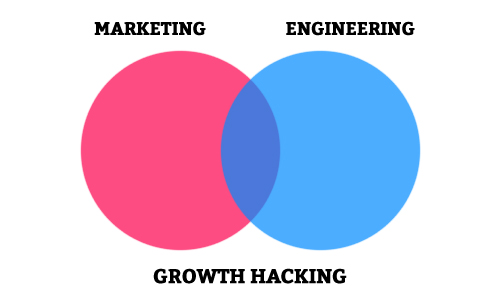
\includegraphics[width=\linewidth]{img/growth-hacker-definition.jpg}
	\caption{Definitie van growth hacking, "Growth hacking as a fusion of two fields"  (Brody 2013, geciteerd 13.05.2016)}
	\label{fig:defGrowthHacker}
\end{figure}

Er zijn overigens geen vaste richtlijnen voor growth hacking, het is een opeenvolging van experimenten die gevoerd wordt om tot de ideale 'hack' te komen. Men moet natuurlijk eerst brainstormen over verschillende mogelijke experimenten. Dat zal een groot deel worden van dit onderzoek; experimenten bedenken en uitwerken die Kriket kan helpen met een versnelde groei.

Om deze experimenten te bedenken zal er eerst een klein marktonderzoek nodig zijn, eventueel door enquêtes of interviews bij andere start-ups en kleine voedselproductie bedrijven. 

Indien mogelijk zou het ook interessant zijn om een experiment uit te voeren en de groei te meten via Google en/of Facebook Analytics. Echter zullen de meeste experimenten theoretisch blijven en zal er door middel van dieper onderzoek een schatting gemaakt worden naar de slaagkansen van het experiment.

%---------- Verwachte resultaten ----------------------------------------------
\section{Verwachte resultaten}
\label{sec:verwachte_resultaten}

De behaalde resultaten zullen voornamelijk bestaan uit enkele uitgewerkte experimenten. Een experiment is dus een mogelijke "hack" die zorgt voor een versnelde community-groei specifiek voor Kriket. 

De enquêtes of interviews van het marktonderzoek kunnen zorgen voor nuttige data die dan in grafieken gebruikt worden.

Indien er een experiment wordt uitgevoerd kan alles gemeten worden via Analytics-tools (zoals eerder vermeld, Google en/of Facebook Analytics). Deze statistieken zullen dan veel inzichten brengen over de hoeveelheid nieuwe bezoekers en klanten, maar ook de weg die ze hebben afgelegd naar Kriket en zoveel meer.


%---------- Verwachte conclusies ----------------------------------------------
\section{Verwachte conclusies}
\label{sec:verwachte_conclusies}

Er wordt verwacht dat het vinden van growth hacking technieken voor een niet-technologische start-up minder conventioneel is dan voor technologische start-ups. Hierdoor zal er dus minder informatie over te vinden zijn en dat maakt dit natuurlijk een zinvol en uitdagend onderzoek.

Uit een uitgevoerd experiment zal hopelijk geconcludeerd kunnen worden dat er een stijging is in het aantal (potentiële) klanten van Kriket, hetzij via Facebook, de website of een reeds eerder vermeld kanaal.

Een groei in de Kriket-community, door dit onderzoek, zou de mooiste conclusie zijn.



%%---------- Andere bijlagen --------------------------------------------------
% TODO: Voeg hier eventuele andere bijlagen toe
%\input{...}

%%---------- Referentielijst --------------------------------------------------

\printbibliography[heading=bibintoc]
%\addcontentsline{toc}{chapter}{\textcolor{maincolor}{\IfLanguageName{dutch}{Bibliografie}{Bibliography}}}

\end{document}
